% \documentclass{article}
\documentclass[a4paper,17pt]{extarticle}
\usepackage[utf8]{inputenc}
\usepackage[document]{ragged2e}
\usepackage{tikz}
\usetikzlibrary{shapes.multipart}
\graphicspath{ {./images/} }
\usepackage{boxhandler}
\setlength{\abovecaptionskip}{8pt}
\usepackage{graphicx, caption}
\usepackage{threeparttable}
\usepackage{xcolor}
\usepackage{scrextend}
\usepackage{titlepic}

\begin{document}

\title{CS 161 P1}
\author{Danny Halawi}
\titlepic{
\begin{figure}[!htb]
\centering

\includegraphics[width=4cm]{me.png}
\caption*{\scriptsize{(pseudonym:\ \textit{dannyallover})}}
\end{figure}
}
\date{October 2020}

\maketitle

\sffamily
\justify
\section*{Question 1: \textit{Tutorial}}
Explanation already done for us in P1 instructions :).\

\subsection*{dejavu.c}
Figure 1 shows the code that we want to exploit, \textit{dejavu.c}.
\begin{figure}[!htb]
  \captionsetup{singlelinecheck = false, format= hang, justification=centering, font=footnotesize, labelsep=space}
  \centering
  \begin{measuredfigure}
    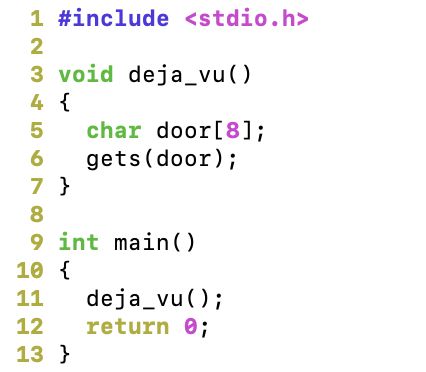
\includegraphics[width=9cm]{q1_dejavu.c.png}
    \caption{\textit{dejavu.c} source code}
  \end{measuredfigure}
  \label{PlP}
\end{figure}

\subsection*{Exploit Script}
Figure 2 highlights the \textit{egg} script, which provides the malicious input to exploit \textit{dejavu.c}.\
\begin{figure}[!htb]
  \captionsetup{singlelinecheck = false, format= hang, justification=centering, font=footnotesize, labelsep=space}
  \centering
  \begin{measuredfigure}
    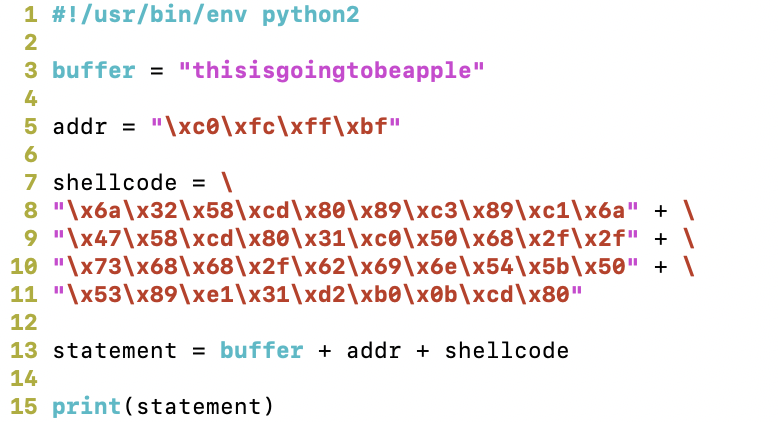
\includegraphics[width=12cm]{q1_egg.png}
    \caption{\textit{egg} script to exploit dejavu.c}
  \end{measuredfigure}
  \label{PlP}
\end{figure}

\section*{Question 2: \textit{Cat vs.\ Dog}}
\subsection*{dog.c}
Figure 3 shows the code that we want to exploit, \textit{dog.c}.
\begin{figure}[!htb]
  \captionsetup{singlelinecheck = false, format= hang, justification=centering, font=footnotesize, labelsep=space}
  \centering
  \begin{measuredfigure}
    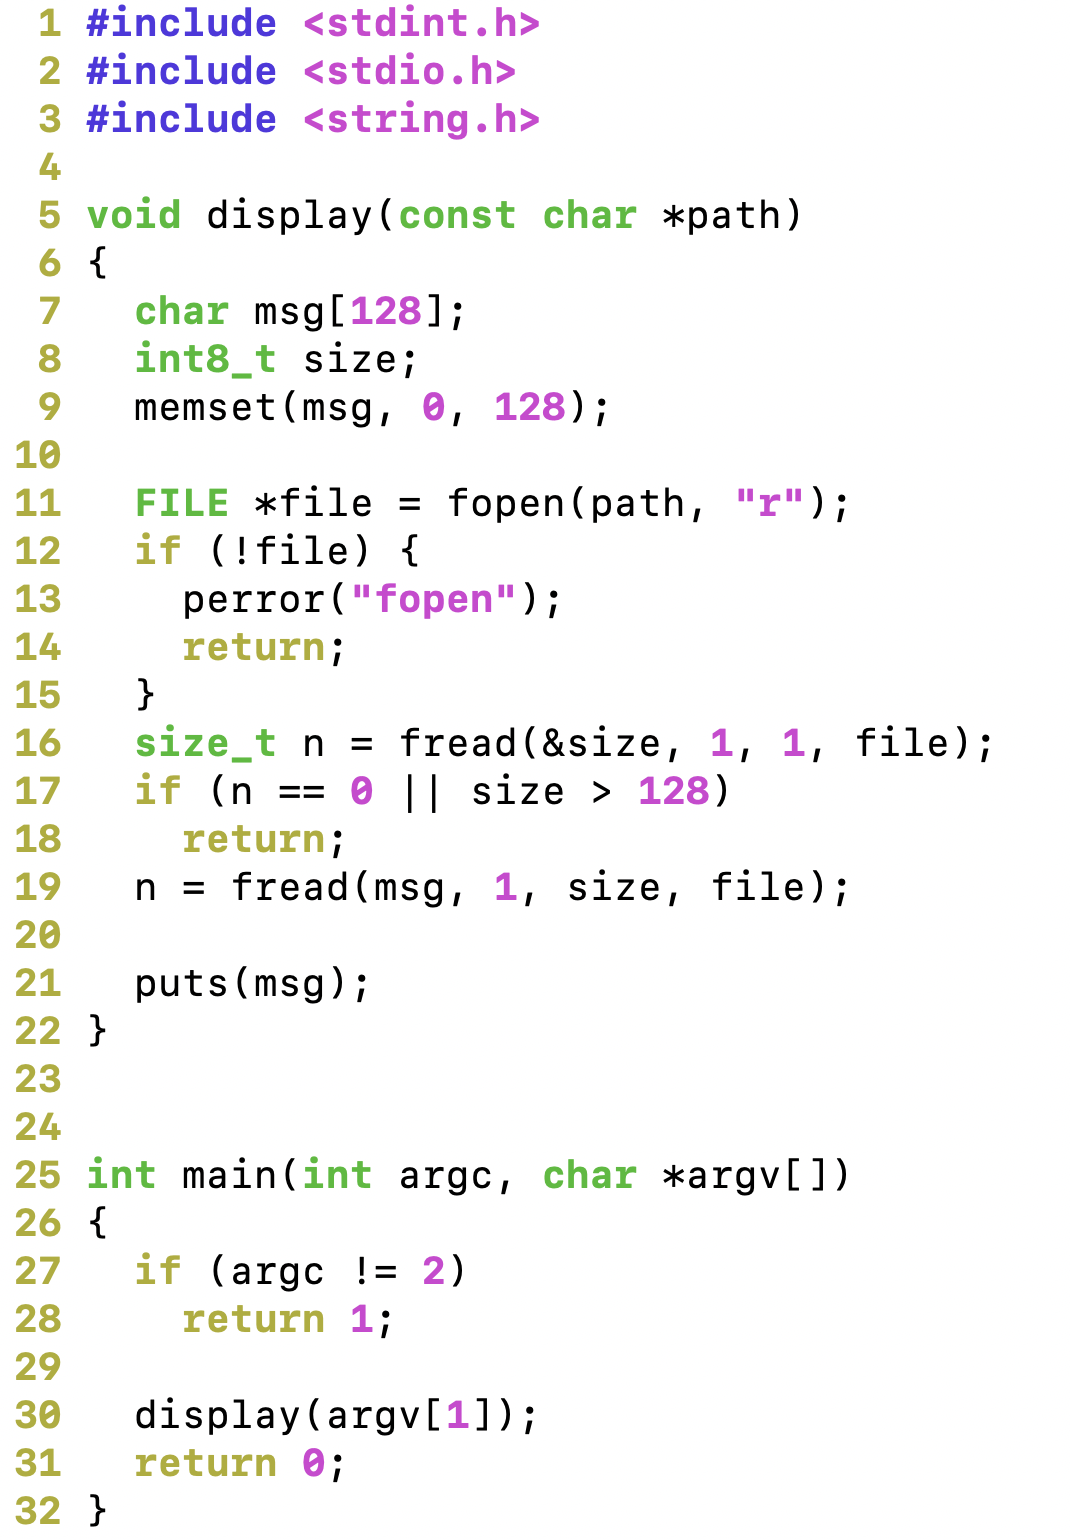
\includegraphics[width=11cm]{q2_dog.c.png}
    \caption{\textit{dog.c} source code}
  \end{measuredfigure}
  \label{PlP}
\end{figure}
\subsection*{Main Idea}
TL;DR:\ The code is vulnerable because of the \textbf{type issue} (i.e.\ unwanted type conversion) that will allows us to \textbf{overflow} the bluffer in \textit{fread}.\
\newline

\noindent
The function \textit{fread} in C takes on the following definition:\ fread(void *ptr, size\_t size, size\_t nmemb, FILE *stream).\
The third argument \textit{nmemb} indicates how many elements to read.\
Notice here, that \textit{nmemb} is of type \textit{size\_t}.\
In the C language, \textit{size\_t} is an unsigned integral type, i.e.\ a typedef (alias) for \textit{unsigned} int in 32 bit systems and \textit{unsigned} long long in 64 bit systems, and, therefore, it cannot be negative.\
Furthermore, when a negative value is assigned to a 
\textit{size\_t} type, it is \textbf{type converted} to an \textit{unsigned} integer.\
\newline

\noindent
To see how we can take advantage of this, let's turn to the code in Figure 3, \textit{dog.c}.\ \underline{Line 8} declares a variable \textit{int8\_t size}, where the type \textit{int8\_t} represents the 8 bit \textit{signed} integers (-128 to 127).\ The question notes that the first byte in the input file is used to indicate the size of the file.\ On \underline{line 16}, that byte is read and assigned to \textit{size}.\ Since one is clever, she can specify a negative number for that one byte.\ This will get past the check on \underline{line 17}, since a negative number will not be equal to 0 or be greater than 128.\ Finally, on \underline{line 19} the negative number \textit{size} is \textbf{type converted} to \textit{size\_t} when passed into \textit{fread}, which when type-converted, can result in a number \textbf{larger} than the file.\ To that end, we are then able to \textbf{write past} the buffer.\
\newline

\noindent
Specifically, we fill the buffer with anything that makes us happy (i.e.\ junk), then overwrite the saved return address on the stack (\textit{rip}) with the address of the shellcode (we'll choose the byte directly after), and insert the shellcode above the \textit{rip} accordingly.\

\subsection*{Magic Numbers}
\begin{figure}[!htb]
  \captionsetup{singlelinecheck = false, format= hang, justification=centering, font=footnotesize, labelsep=space}
  \centering
  \begin{measuredfigure}
    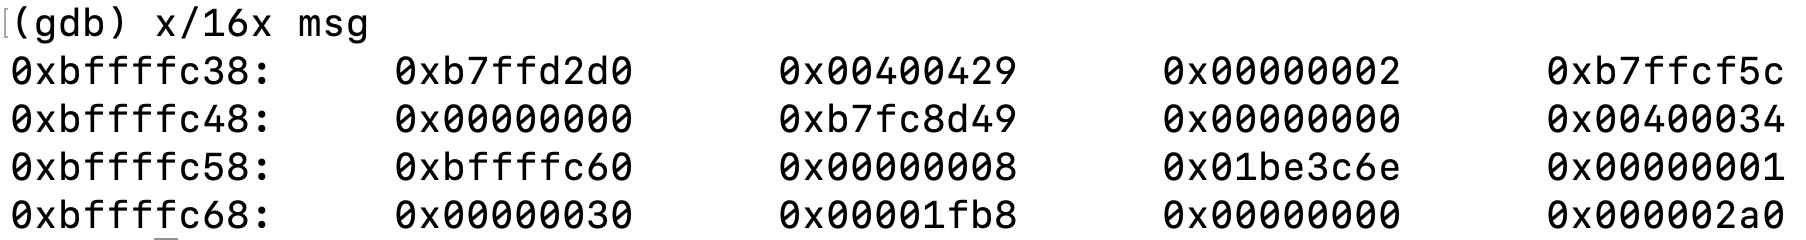
\includegraphics[width=12cm]{q2_buf.png}
    \caption{sixteen bytes starting at \textit{msg} buffer in \textit{display} function}
  \end{measuredfigure}
  \label{PlP}
\end{figure}

\noindent
First, we determine the address of the buffer, \textit{msg}.\ To do this, we open up GDB and place a break at \underline{line 7}, \textcolor{gray}{b 7}.\ By running the program, hitting the break, and then using the command \textcolor{gray}{x/16x msg} (print sixteen bytes starting at \textit{msg}), we determine the address of the buffer:\ \underline{0xbffffc38}, seen in Figure 4.\
\newline

\begin{figure}[!htb]
  \captionsetup{singlelinecheck = false, format= hang, justification=centering, font=footnotesize, labelsep=space}
  \centering
  \begin{measuredfigure}
    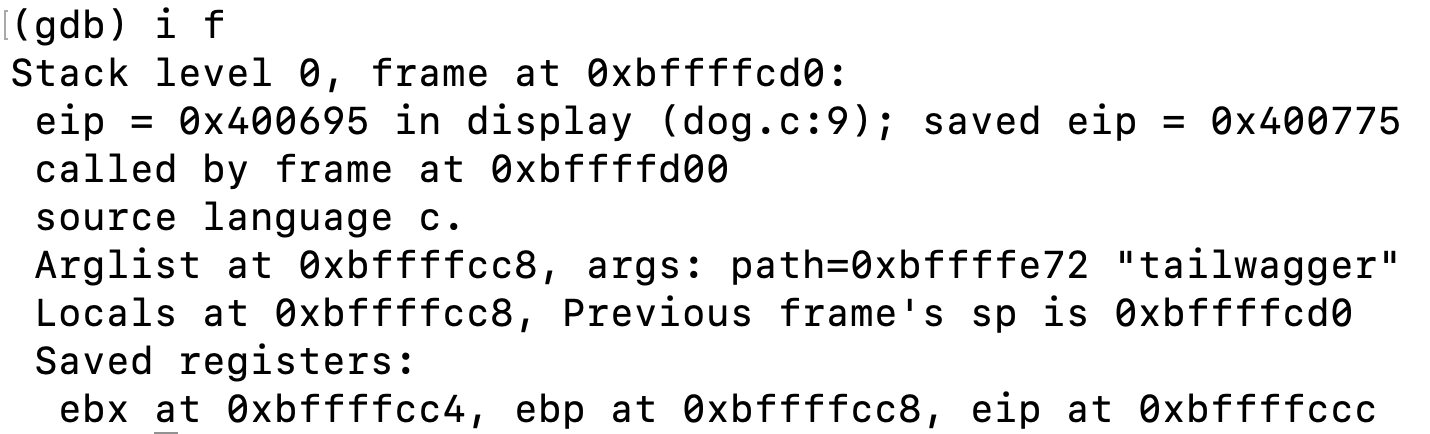
\includegraphics[width=12cm]{q2_eip.png}
    \caption{address of saved \textit{eip} (\textit{rip}) in \textit{display} function}
  \end{measuredfigure}
  \label{PlP}
\end{figure}

\noindent
Next, we determine the location of the saved \textit{eip} (\textit{rip}) for the function we want to exploit, \textit{display}.\ By using the break statement on \underline{line 7} and the command \textcolor{gray}{i f} (display information about the frame), we see \textit{eip} was stored at address \underline{0xbffffccc}, shown in\ Figure 5.
\newline

\noindent
By doing so, we learned that the location of the return address from this function is
\underline{148} bytes away from the start of the \textit{msg} buffer (\underline{0xbffffccc $-$ 0xbffffc38 $=$ 0x94 $=$ 148}).
\newline

\noindent
Lastly, the total size of the file is going to take on the following sum:\ 128 bytes (for overwriting \textit{msg}) + 20 bytes (for overwriting everything up until \textit{rip}) + 4 bytes (for overwriting \textit{rip}) + 39 bytes (for shellcode) = \underline{191} bytes = \underline{0xbf}.\ Therefore, we assign \underline{0xbf} as the size of the file.\ The magic is here is that when \underline{0xbf} is fed into \textit{int8\_t size}, it will be interpreted as a negative number, since it exceeds the positive integer limit of 127.

\subsection*{Exploit Structure}
Figure 6 paints the stack diagram before the exploit.
\begin{figure}[!htb]
  \captionsetup{singlelinecheck = false, format= hang, justification=centering, font=footnotesize, labelsep=space}
  \centering
  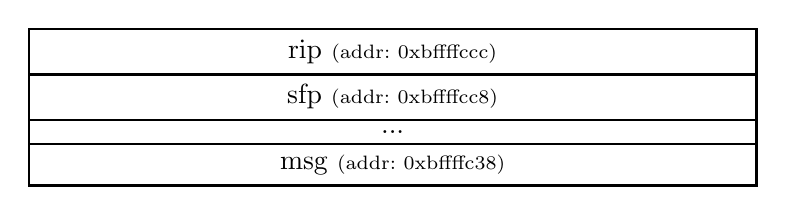
\begin{tikzpicture}[stack/.style={rectangle split, rectangle split parts=#1,draw, anchor=center}]
  \node[stack=4, line width=1pt, text width=9cm, text centered]  {
  \nodepart{one}rip \scriptsize(addr:\ 0xbffffccc)
  \nodepart{two}sfp \scriptsize(addr:\ 0xbffffcc8)
  \nodepart{three}...
  \nodepart{four}msg \scriptsize(addr:\ 0xbffffc38)
  };
  \end{tikzpicture}
  \caption{stack diagram before exploit}
  \label{PlP}
\end{figure}

\noindent
The exploit has four parts:
\begin{addmargin}[1em]{2em}
1.\ Feed \underline{0xbf} as the first byte to indicate the size of the file.
\newline
\noindent
2.\ Feed \underline{148} bytes of junk to overwrite the buffer, everything in-between, and the \textit{sfp}.
\newline
\noindent
3.\ Overwrite the \textit{rip} with the address of the shellcode.\ Since we are putting the shellcode directly after the \textit{rip}, we overwrite the \textit{rip} with \underline{0xbffffcd0} (\underline{0xbffffccc + 4}).\
\newline
\noindent
4.\ Finally, insert the shellcode directly after the \textit{rip}.\
\end{addmargin}

\begin{figure}[!htb]
  \captionsetup{singlelinecheck = false, format= hang, justification=centering, font=footnotesize, labelsep=space}
  \centering
  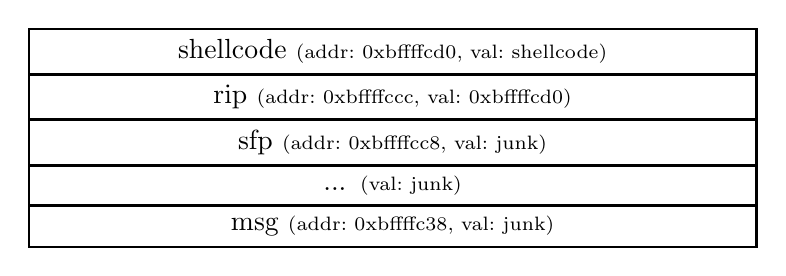
\begin{tikzpicture}[stack/.style={rectangle split, rectangle split parts=#1,draw, anchor=center}]
  \node[stack=5, line width=1pt, text width=9cm, text centered]  {
  \nodepart{one}shellcode \scriptsize(addr:\ 0xbffffcd0, val:\ shellcode)
  \nodepart{two}rip \scriptsize(addr:\ 0xbffffccc, val:\ 0xbffffcd0)
  \nodepart{three}sfp \scriptsize(addr:\ 0xbffffcc8, val:\ junk)
  \nodepart{four}... \scriptsize(val:\ junk)
  \nodepart{five}msg \scriptsize(addr:\ 0xbffffc38, val:\ junk)
  };
  \end{tikzpicture}
  \caption{stack diagram after buffer overflow}
  \label{PlP}
\end{figure}

\noindent
Figure 7 reflects the stack diagram once the input of the exploit is fed in.\ This causes the \textit{display} function to start executing the shellcode at address \underline{0xbffffcd0} upon return.\

\subsection*{Exploit GDB Output}
\begin{figure}[!htb]
  \captionsetup{singlelinecheck = false, format= hang, justification=centering, font=footnotesize, labelsep=space}
  \centering
  \begin{measuredfigure}
    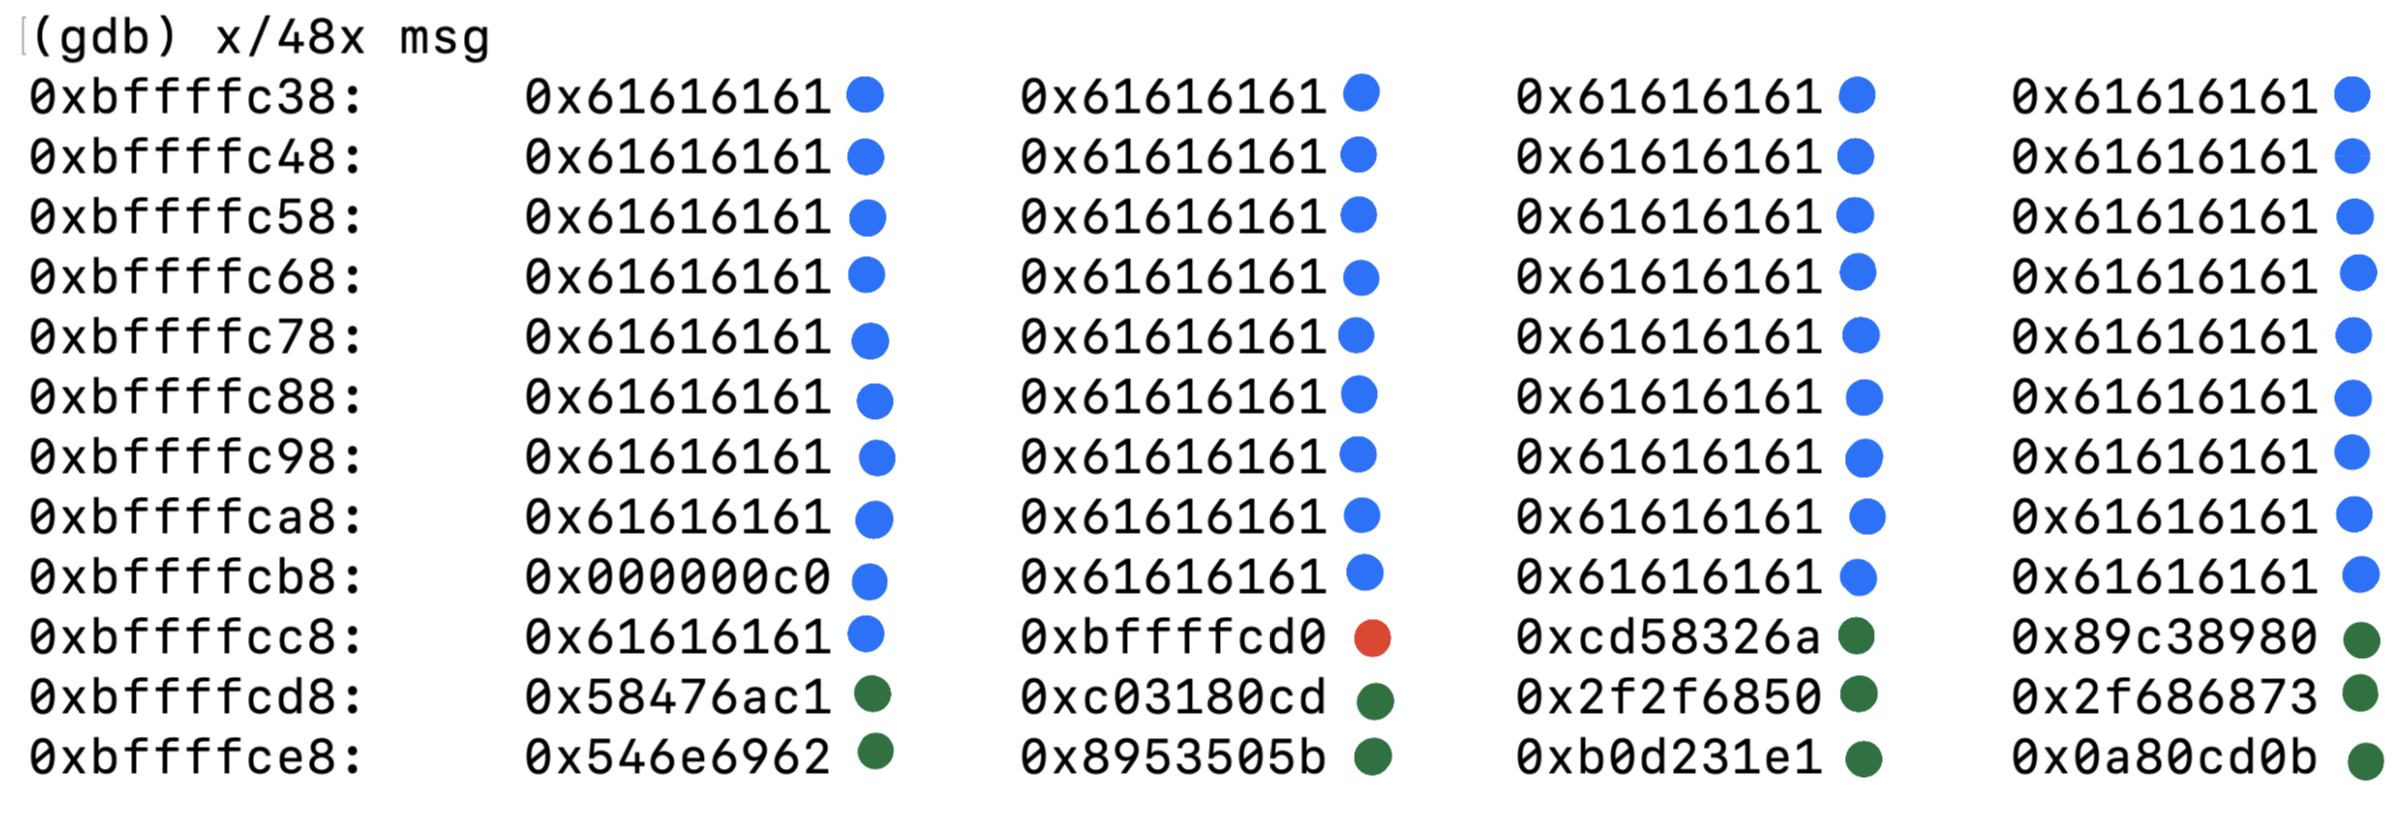
\includegraphics[width=12cm]{q2_output.png}
    \caption{GDB output after feeding exploit string}
  \end{measuredfigure}
    \label{PlP}
\end{figure}
\noindent
Figure 8 highlights the GDB output after inputting the malicious exploit string.\ After \underline{148} bytes of garbage (blue), the \textit{rip} (red) is overwritten with \underline{0xbffffcd0}, which points to the shellcode (green), which is directly after the \textit{rip}.\

\subsection*{Exploit Script}
Figure 9 highlights the \textit{egg} script, which provides the malicious input to exploit \textit{dog.c}.\
\begin{figure}[!htb]
  \captionsetup{singlelinecheck = false, format= hang, justification=centering, font=footnotesize, labelsep=space}
  \centering
  \begin{measuredfigure}
    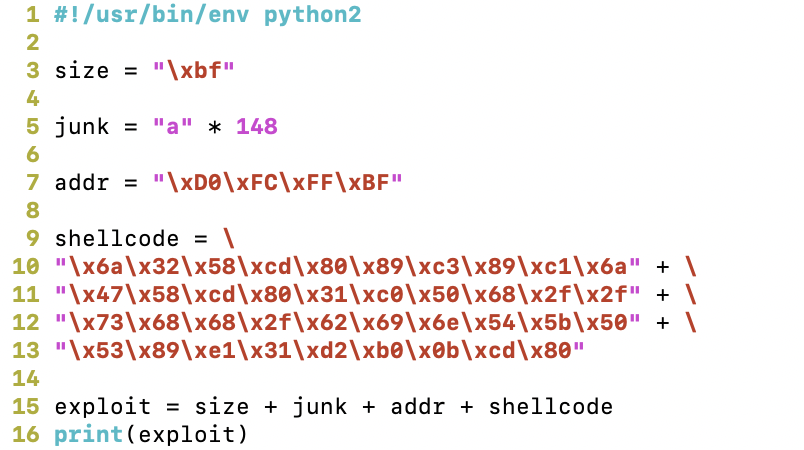
\includegraphics[width=12cm]{q2_egg.png}
    \caption{\textit{egg} script to exploit \textit{dog.c}}
  \end{measuredfigure}
  \label{PlP}
\end{figure}


\section*{Question 3: \textit{Advance Warning}}
\subsection*{dehexify.c}
Figure 10 shows the code that we want to exploit, \textit{dehexify.c}.\
\begin{figure}[!htb]
  \captionsetup{singlelinecheck = false, format= hang, justification=centering, font=footnotesize, labelsep=space}
  \centering
  \begin{measuredfigure}
    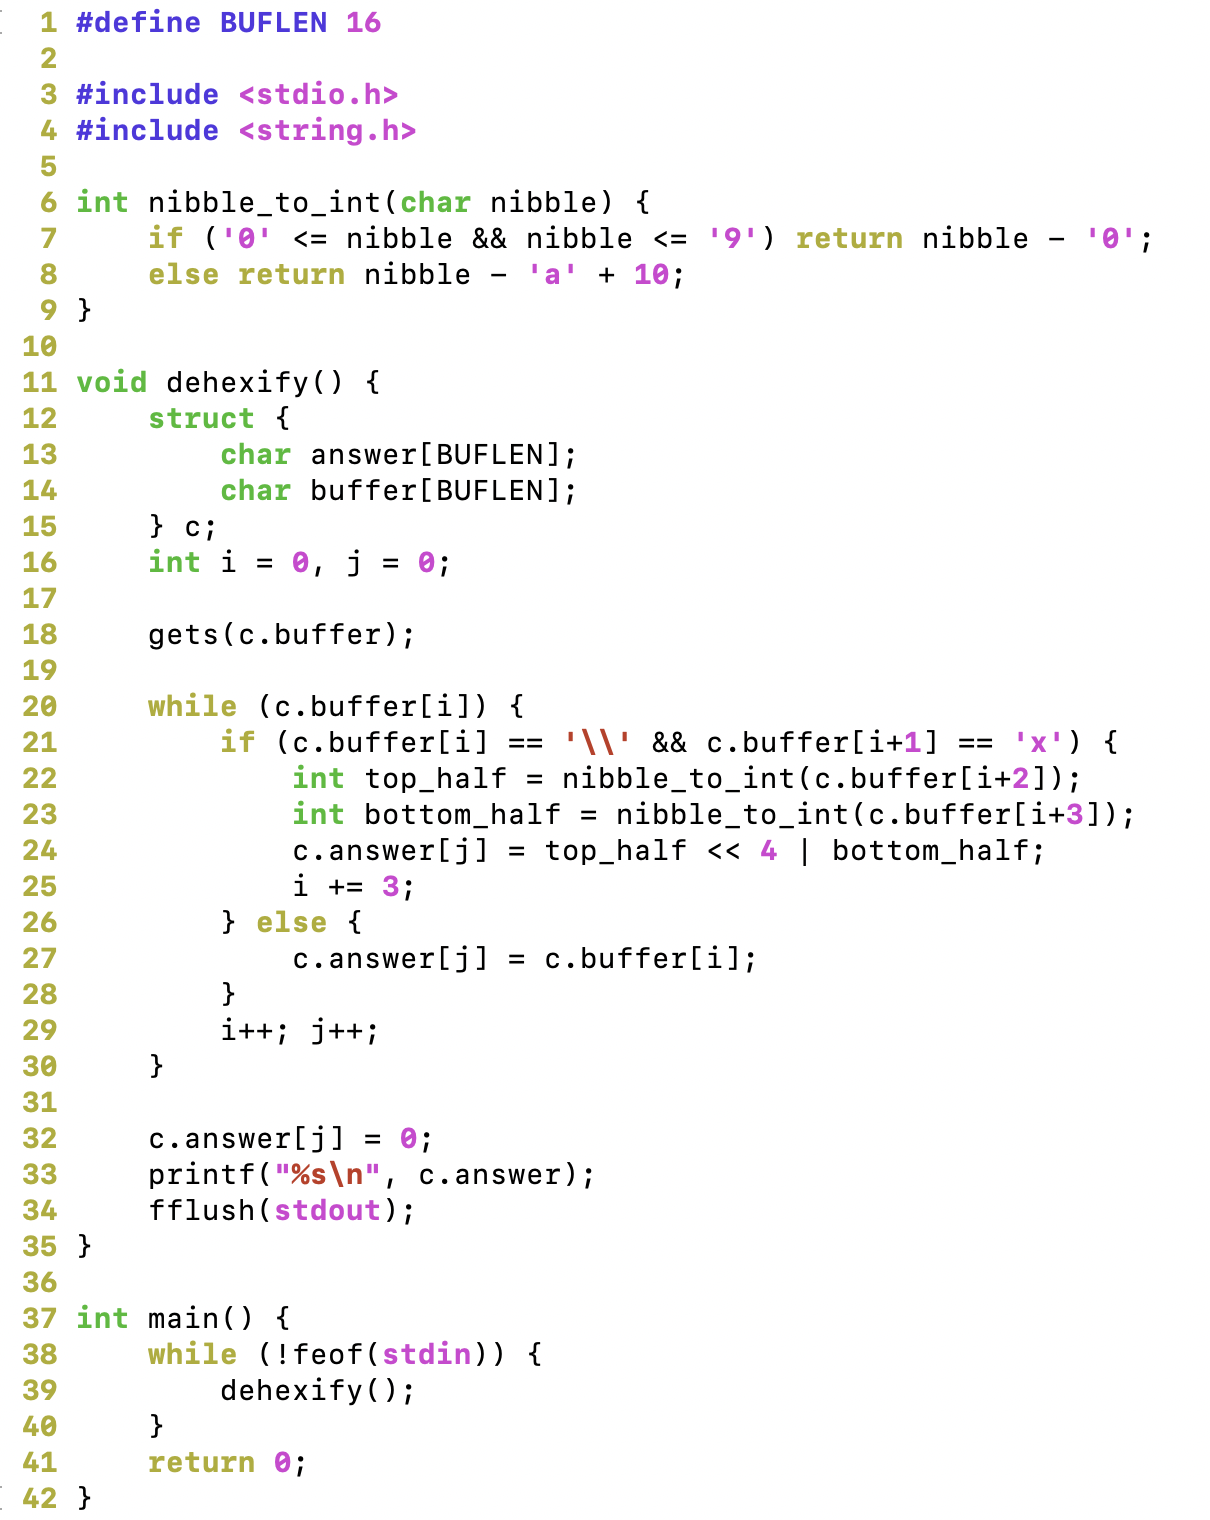
\includegraphics[width=12cm]{q3_dehexify.png}
    \caption{\textit{dehexify.c} source code}
  \end{measuredfigure}
  \label{PlP}
\end{figure}
\subsection*{Main Idea}
TL;DR:\ The code is vulnerable because the lack of \textbf{bounds check} allows us to read past the buffer when \underline{line 25} (\textit{i += 3}) and then \underline{line 29} (\textit{i++}) are executed to skip the null bytes in the buffer, which can be leveraged to \textbf{extract the canary}.\ Then, \textit{gets(door)} does not check the length of the input from the user, which allows us to \textbf{overflow} the buffer (\textbf{making sure to overwrite the canary with itself}).\
\newline

\noindent
The program has the \textbf{stack-canary} enabled.\ Therefore, when we write past the buffer and hit the canary, we must overwrite the canary with itself; otherwise, the program will intently crash.\
\newline

\noindent
First, we want to make sure to provide input that will not overwrite the canary, i.e.\ we have to stay within the \textit{BUFLEN} of \underline{16 bytes}.\ Furthermore, in the problem, it says that \textit{gets} will append two null bytes to the input.\ Therefore, we'll want to leverage the code to skip the null-bytes so that the \textit{while} loop on \underline{line 20} does not terminate at the end of \textit{buffer}.\ By feeding in the proper characters, we can enter the if statement on \underline{line 21} and skip the null-bytes when \underline{line 25} (\textit{i += 3}) is executed follow by \underline{line 29} (\textit{i++}).\ This will allow us to read the canary into \textit{c.answer} on \underline{line 27}, which is then printed out on \underline{line 33} for us to retrieve.\
\newline

\noindent
Further, once the canary is retrieved.\ We use the fact that \textit{gets(door)} does not check the length of the input from the user (keeps getting until \textit{new-line} character) to write as much as we want and overflow the buffer.\
\newline

\noindent
Specifically, we fill the buffer with anything that makes us happy (i.e.\ junk), overwrite the canary with itself, overwrite the saved return address on the stack (\textit{rip}) with the address of the shellcode (we'll choose the byte directly after), and insert the shellcode above the \textit{rip} accordingly.\

\subsection*{Magic Numbers}
\begin{figure}[!htb]
  \captionsetup{singlelinecheck = false, format= hang, justification=raggedright, font=footnotesize, labelsep=space}
  \centering
  \begin{measuredfigure}
    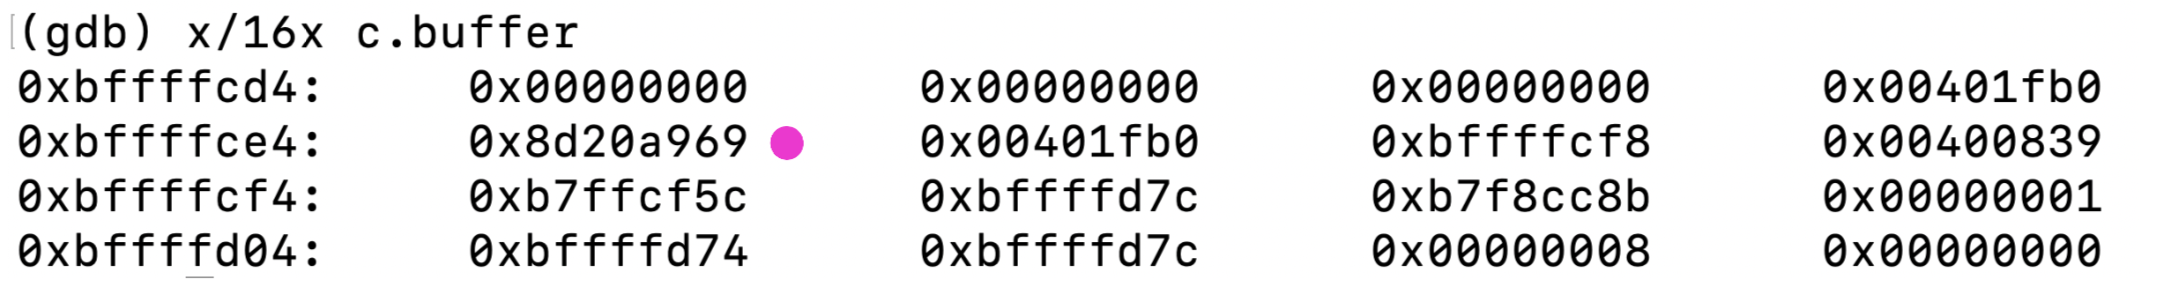
\includegraphics[width=12cm]{q3_canary_loc_1.png}
    \caption{sixteen bytes starting at \textit{c.buffer} in \textit{dehexify} function (pass 1)}
  \end{measuredfigure}
  \label{PlP}
\end{figure}
\begin{figure}[!htb]
  \captionsetup{singlelinecheck = false, format= hang, justification=raggedright, font=footnotesize, labelsep=space}
  \centering
  \begin{measuredfigure}
    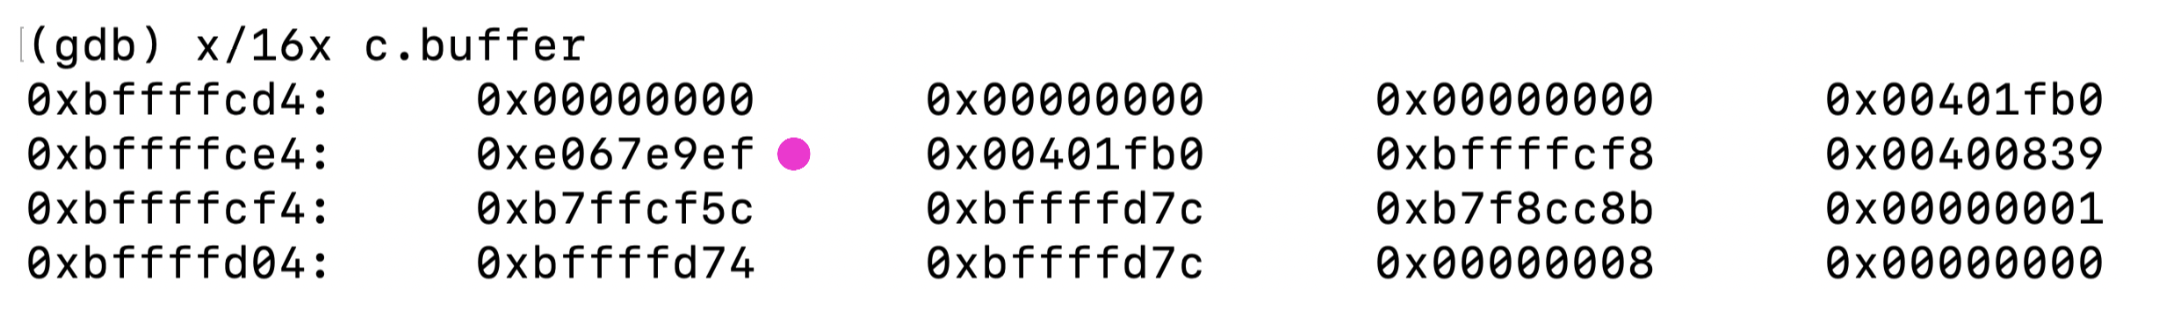
\includegraphics[width=12cm]{q3_canary_loc_2.png}
    \caption{sixteen bytes starting at \textit{c.buffer} in \textit{dehexify} function (pass 2)}
  \end{measuredfigure}
  \label{PlP}
\end{figure}

\noindent
First, we must determine the address of the canary in the function we want to exploit, \textit{dehexify}.\
We suspect the canary is going to be above the locals on the stack.\ Therefore, we take the highest local variable on the stack \textit{c.buffer} and observe the values after it to see what constantly changes (since we know the canary, by nature, will change every time).\ To do this, we open up GDB and place a break at \underline{line 12}, \textcolor{gray}{b 12}.\ By running the program, hitting the break, and then using the command \textcolor{gray}{x/16x c.buffer}, we can look for the value that changes.\ Figures 11 and 12 show that the value at address \underline{0xbffffce4} changes.\ We conclude that is the location of the canary.\
\newline

\begin{figure}[!htb]
  \captionsetup{singlelinecheck = false, format= hang, justification=centering, font=footnotesize, labelsep=space}
  \centering
  \begin{measuredfigure}
    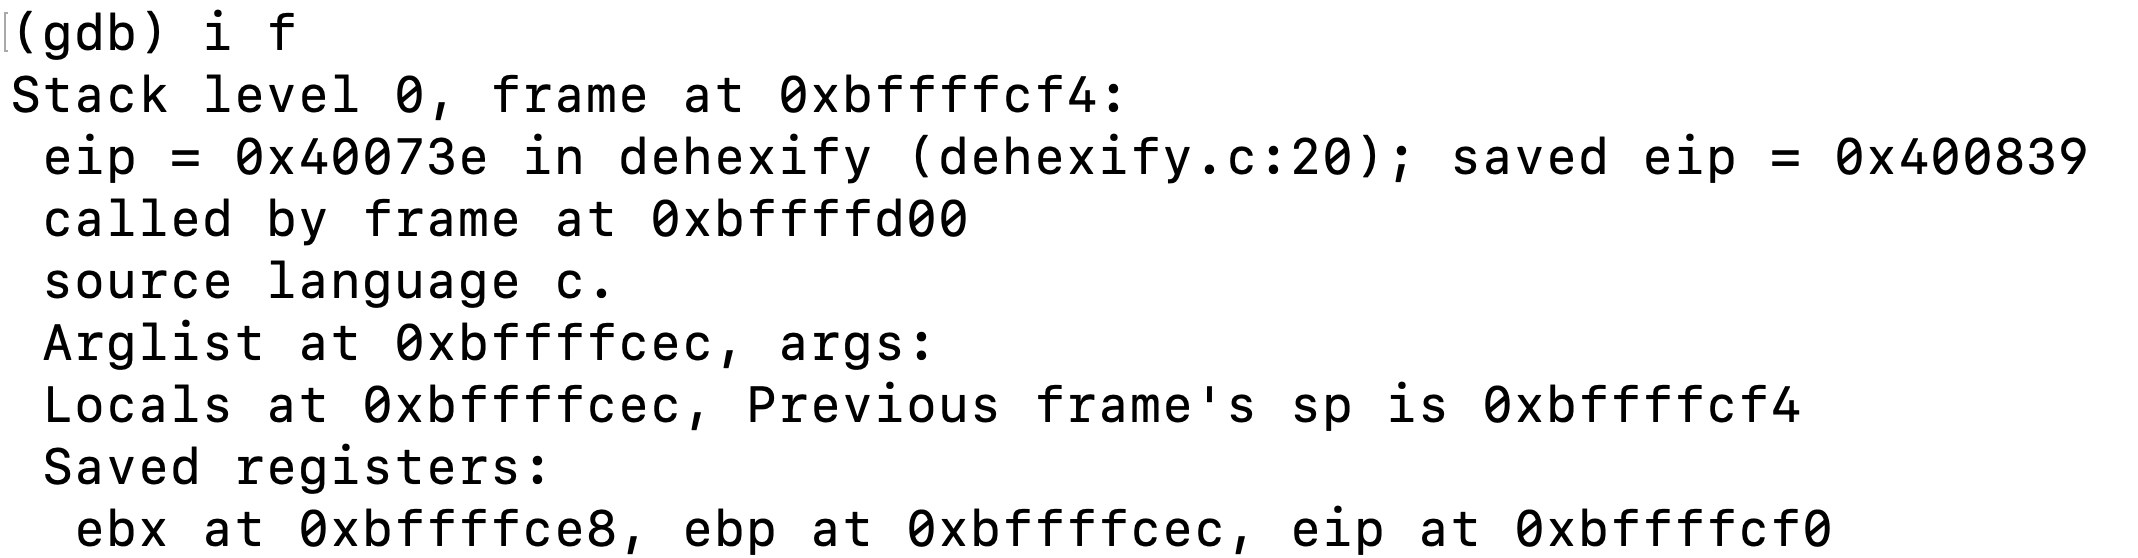
\includegraphics[width=12cm]{q3_eip.png}
    \caption{address of saved \textit{eip} (\textit{rip}) in \textit{dehexify} function}
  \end{measuredfigure}
  \label{PlP}
\end{figure}

\noindent
Next, we determine the location of the saved \textit{eip} (\textit{rip}) for the function we want to exploit, \textit{dehexify}.\ By using the break statement on \underline{line 12} and the \textcolor{gray}{i f} command, we see \textit{eip} was stored at the address \underline{0xbffffcf0}, shown in Figure 13.\ Additionally, Figure 11 points out that the address of \textit{c.buffer} is \underline{0xbffffcd4}.\ Therefore, we learned that the location of the return address from this function is \underline{28} bytes from the start of \textit{buffer} (\underline{0xbffffcf0 $-$ 0xbffffcd4 $=$ 0x1c = 28}).\

\subsection*{Exploit Structure}
Figure 14 paints the stack diagram before the exploit.
\newline
\begin{figure}[!htb]
  \captionsetup{singlelinecheck = false, format= hang, justification=centering, font=footnotesize, labelsep=space}
  \centering
  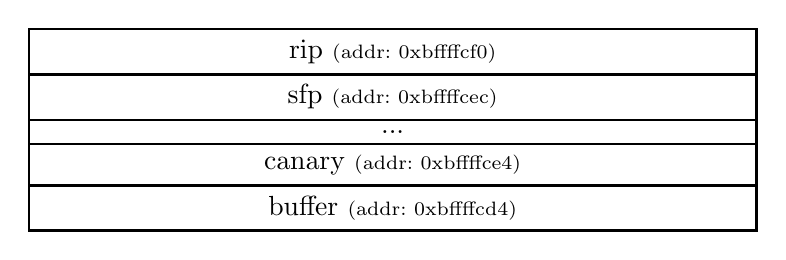
\begin{tikzpicture}[stack/.style={rectangle split, rectangle split parts=#1,draw, anchor=center}]
  \node[stack=5, line width=1pt, text width=9cm, text centered]  {
  \nodepart{one}rip \scriptsize(addr:\ 0xbffffcf0)
  \nodepart{two}sfp \scriptsize(addr:\ 0xbffffcec)
  \nodepart{three}...
  \nodepart{four}canary \scriptsize(addr:\ 0xbffffce4)
  \nodepart{five}buffer \scriptsize(addr:\ 0xbffffcd4)
  };
  \end{tikzpicture}
  \caption{stack diagram before exploit}
  \label{PlP}
\end{figure}

\noindent
The exploit takes on the following procedure.
\newline
\noindent
First-pass (get the canary):
\begin{addmargin}[1em]{2em}
1.\ Feed \underline{12} bytes of junk followed by 
'\textbackslash\textbackslash', 'x', and the new-line character '\textbackslash n' (to terminate \textit{gets}).\ This specific inputs feeds in \underline{14} bytes + the \underline{2} appended null-bytes by \textit{get} (does not overwrite the canary).\ Furthermore, when \textit{i} is equal to \underline{12}, we can properly enter the \textit{if} statement on \underline{line 21} and then, as described above, skip the null-bytes by getting \textit{i} to increment to \underline{16} with \underline{lines 25 and 29}.\ This will allow us to read the canary into \textit{c.answer} on \underline{line 27}, which is then printed out on \underline{line 33} for us to retrieve.\ (note:\ one need not worry about an infinite loop, since Figures 11 and 12 highlight that there is a null byte after the canary).\
\end{addmargin}

\noindent
Second-pass (use the canary \& overflow the buffer):
\begin{addmargin}[1em]{2em}
1.\ Overwrite \textit{buffer} with \underline{15} bytes of junk followed by a null-byte (\underline{1} byte) since we don't want to stay in the loop this time (specifically, if we're in the loop past the buffer length (\textit{BUFLEN}), \underline{line 27} will potentially give us issues by overwriting our malicious input if it goes far enough).
\newline
\noindent
2.\ Overwite the canary (retrieved in the first-pass) with itself.
\newline
\noindent
3.\ We know that \textit{rip} is \underline{28} bytes away from the start of buffer, so we feed \underline{8} more bytes of junk, overwriting \textit{sfp} and everything in between.
\newline
\noindent
4.\ Overwrite \textit{rip} the address of the shellcode.\ Since we are putting the shellcode directly after the \textit{rip}, we overwrite the \textit{rip} with \underline{0xbffffcf4} (\underline{0xbffffcf0 + 4}).\
\newline
\noindent
5.\ Finally, insert the shellcode directly after the \textit{rip}.
\newline
\end{addmargin}

\begin{figure}[!htb]
  \captionsetup{singlelinecheck = false, format= hang, justification=centering, font=footnotesize, labelsep=space}
  \centering
  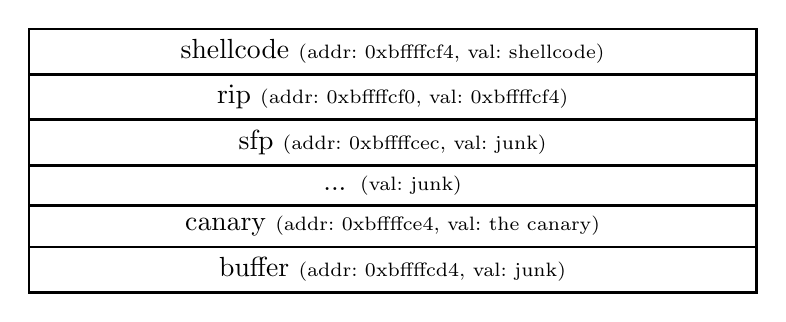
\begin{tikzpicture}[stack/.style={rectangle split, rectangle split parts=#1,draw, anchor=center}]
  \node[stack=6, line width=1pt, text width=9cm, text centered]  {
  \nodepart{one}shellcode \scriptsize(addr:\ 0xbffffcf4, val:\ shellcode)
  \nodepart{two}rip \scriptsize(addr:\ 0xbffffcf0, val:\ 0xbffffcf4)
  \nodepart{three}sfp \scriptsize(addr:\ 0xbffffcec, val:\ junk)
  \nodepart{four}... \scriptsize(val:\ junk)
  \nodepart{five}canary \scriptsize(addr:\ 0xbffffce4, val:\ the canary)
  \nodepart{six}buffer \scriptsize(addr:\ 0xbffffcd4, val:\ junk)
  };
  \end{tikzpicture}
  \caption{stack diagram after buffer overflow}
  \label{PlP}
\end{figure}

\noindent
Figure 15 reflects the stack diagram once the input of the exploit is fed in.\ This causes the \textit{dehexify} function to execute the shellcode at \underline{0xbffffcf4} upon return.

\subsection*{Exploit GDB Output}
Figure 16 shows the value of \textit{c.buffer} after the first \textit{p.send}.\ We see that we have 16 bytes of junk (blue), followed by the canary (pink).\ In particular, the last byte of \textit{buf} is \underline{0x0000785c} which is equivalent to '\textbackslash\textbackslash' (\underline{0x5c}), 'x' (\underline{0x78}), null-byte (\underline{0x00}), and null-byte (\underline{0x00}), as desired.
\newline

\begin{figure}[!htb]
  \captionsetup{singlelinecheck = false, format= hang, justification=centering, font=footnotesize, labelsep=space}
  \centering
  \begin{measuredfigure}
    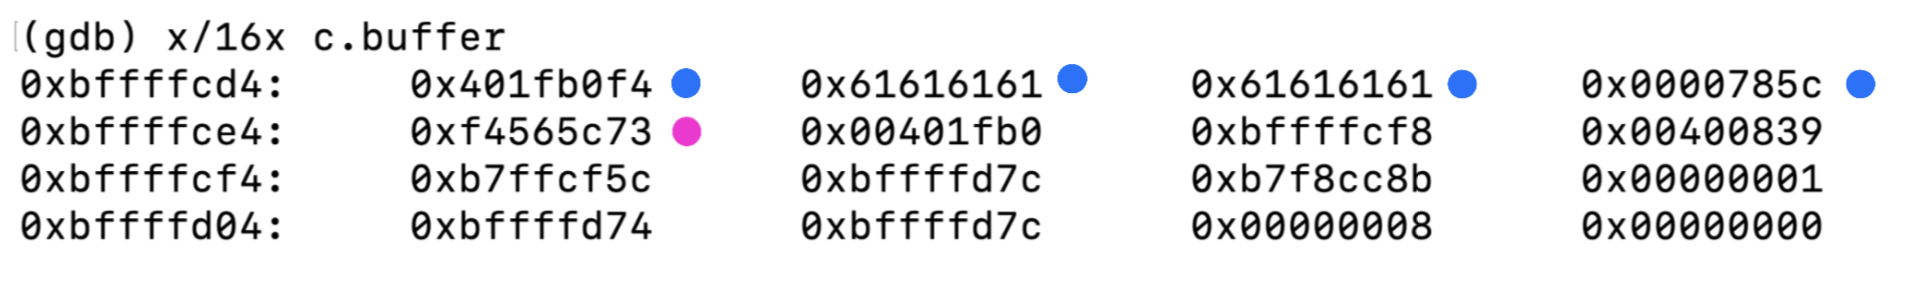
\includegraphics[width=12cm]{q3_canary_in_answer_1.png}
    \caption{\textit{c.buffer} after first \textit{p.send}}
  \end{measuredfigure}
  \label{PlP}
\end{figure}

\noindent
Figure 17 shows that the value of the canary is successfully written in \textit{c.answer} after we execute the loop.
\newline

\begin{figure}[!htb]
  \captionsetup{singlelinecheck = false, format= hang, justification=raggedright, font=footnotesize, labelsep=space}
  \centering
  \begin{measuredfigure}
    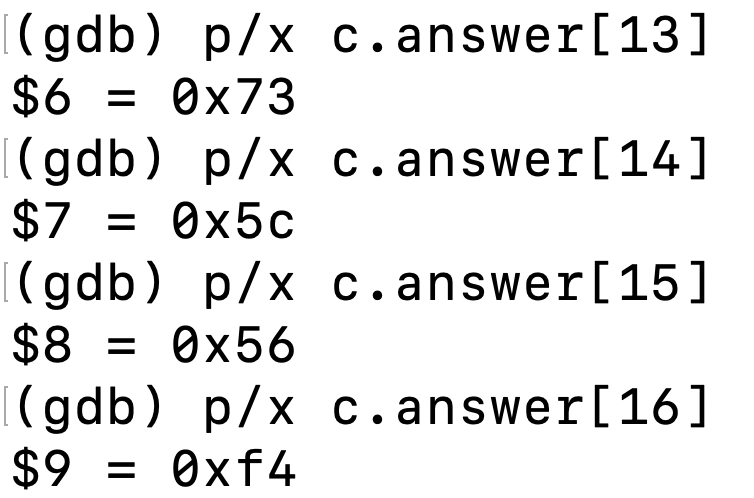
\includegraphics[width=4cm]{q3_canary_in_answer_2.png}
    \caption{value of the canary in \textit{c.answer}}
  \end{measuredfigure}
  \label{PlP}
\end{figure}

\noindent
According to Nicholas Ngai, "Since it is hard to show the GDB output after the second p.send, we accept a stack diagram in place of the second GDB output resulting from the second p.send".\ Furthermore, one can see such stack diagram in the previous section.

\subsection*{Exploit Script}
Figure 18 highlights the \textit{interact} script, which executes the exploit of \textit{dehexify.c}.
\begin{figure}[!htb]
  \captionsetup{singlelinecheck = false, format= hang, justification=centering, font=footnotesize, labelsep=space}
  \centering
  \begin{measuredfigure}
    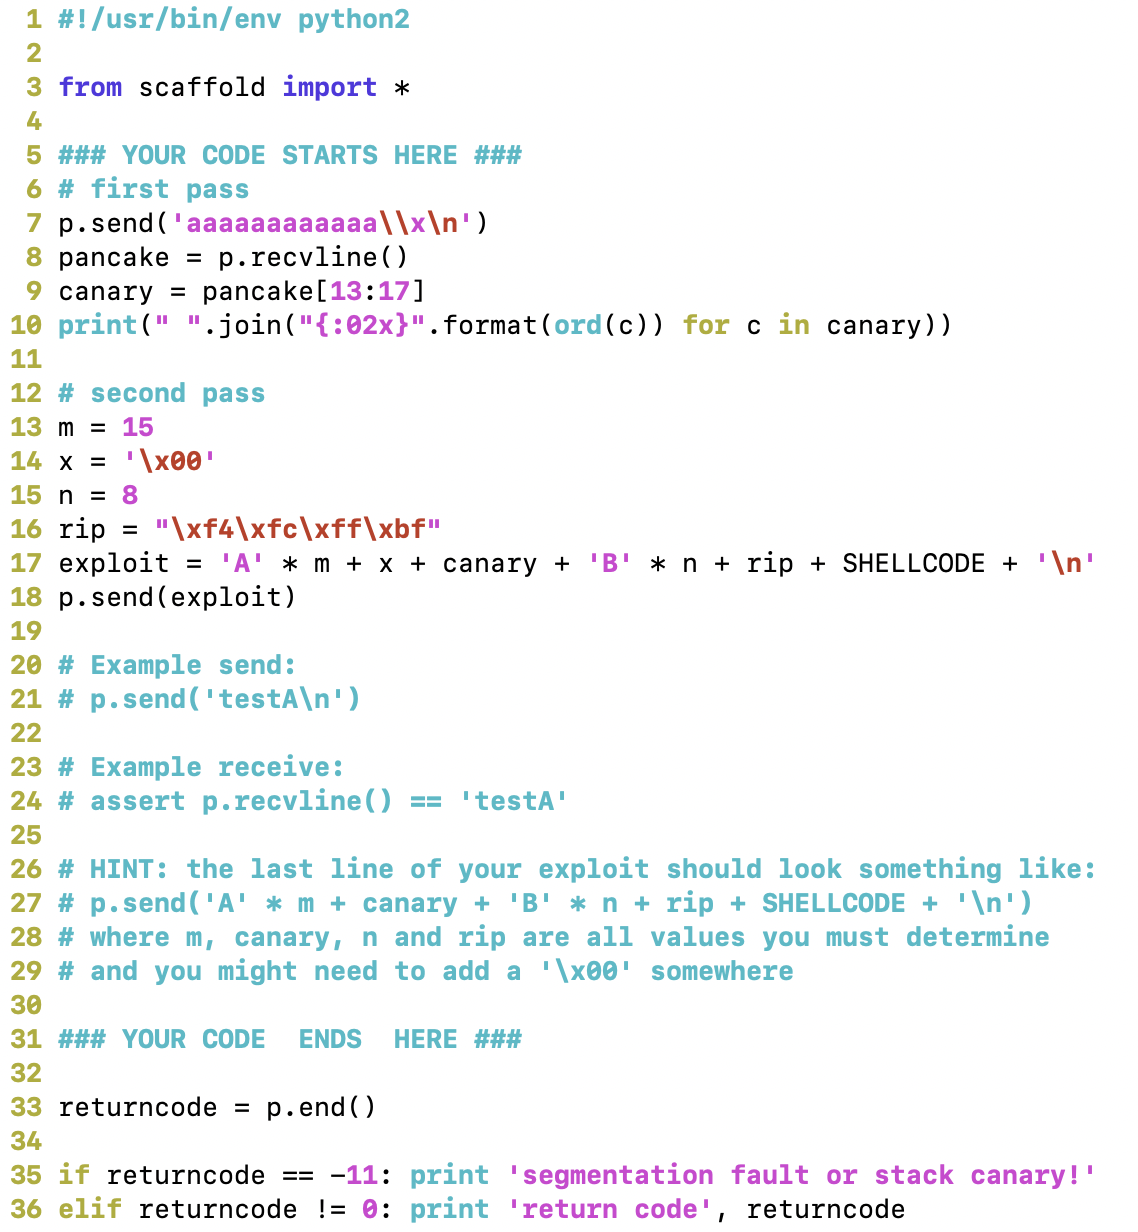
\includegraphics[width=10cm]{q3_interact.png}
    \caption{\textit{interact} script to exploit dehexify.c}
  \end{measuredfigure}
  \label{PlP}
\end{figure}

\section*{Question 4: Stack Flipper}
\subsection*{flipper.c}
Figure 19 shows the code that we want to exploit, \textit{flipper.c}.
\begin{figure}[!htb]
  \captionsetup{singlelinecheck = false, format= hang, justification=centering, font=footnotesize, labelsep=space}
  \centering
  \begin{measuredfigure}
    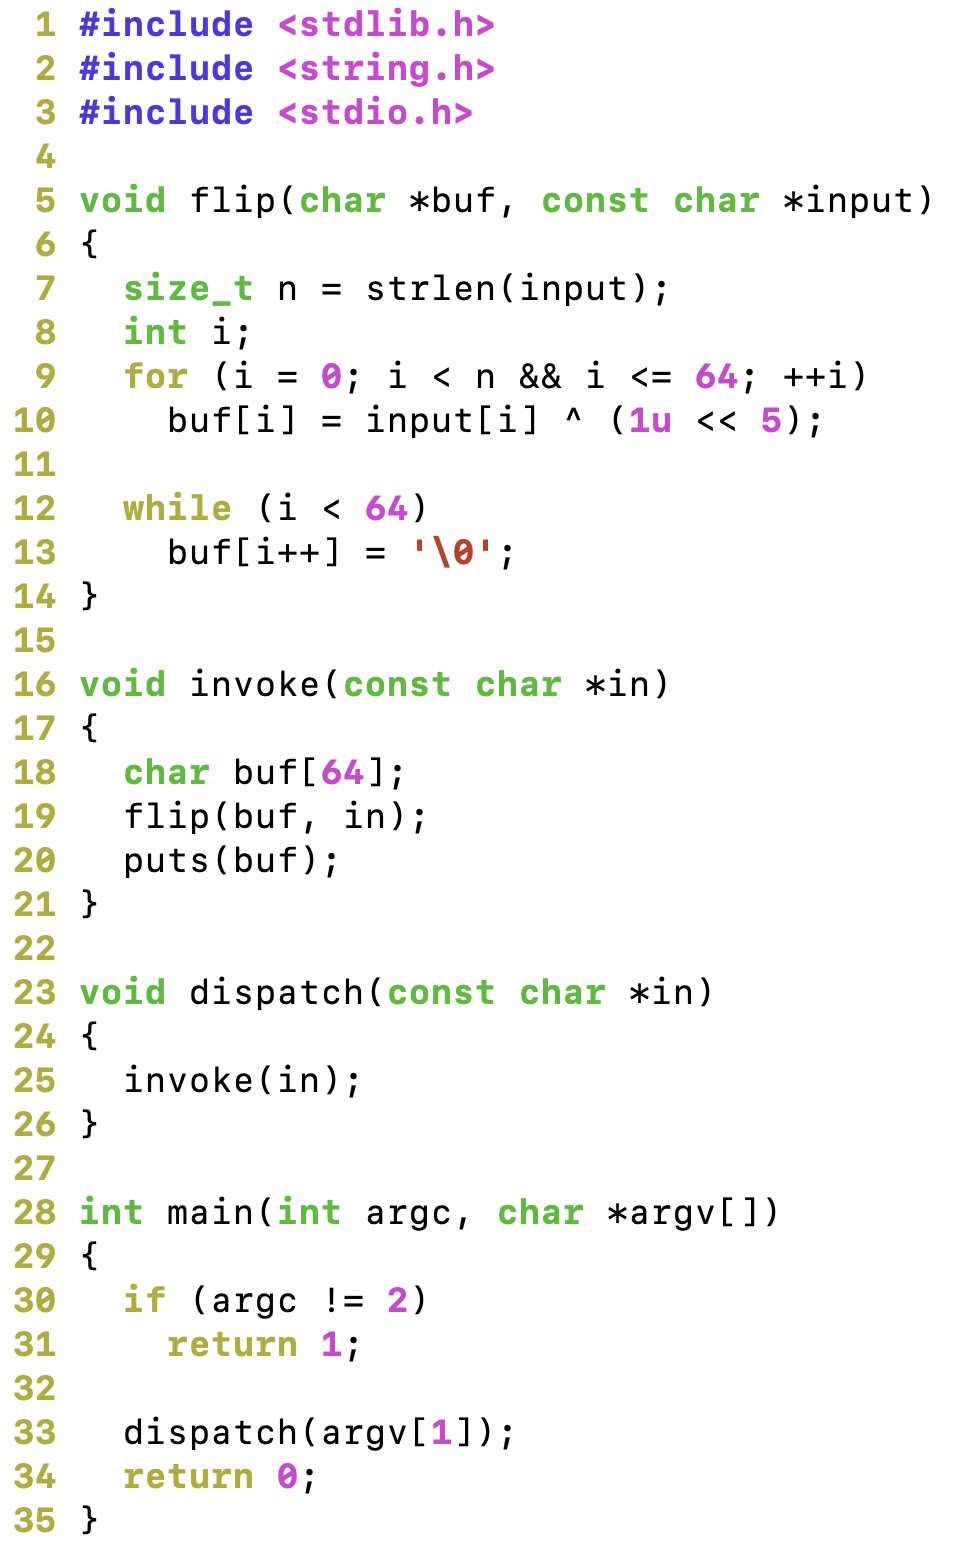
\includegraphics[width=9cm]{q4_flipper.c.png}
    \caption{\textit{flipper.c} source code}
  \end{measuredfigure}
  \label{PlP}
\end{figure}
\subsection*{Main Idea}
TL;DR:\ The code is vulnerable because of an \textbf{off-by-one} error.\ The \textit{for} loop does not have the proper \textbf{bounds check}, which allows us to write one byte \textbf{past the buffer}.\ Since the \textit{esp} is right after the buffer, we can overwrite the last byte (least significant byte) of \textit{esp} to point inside the buffer.\ We write the address of our environment variable (shellcode) in our buffer, which will eventually result in the execution of our shellcode (through the steps outlined below).
\newline
 
\noindent
I'm going to describe in detail the method of exploitation.\ The ideas here are a summary of Section 10 of \textit{ASLR Smack \& Laugh Reference} by Tilo M\"uller.\ According to instructor EvanBot on Piazza, "OSINT is accepted if source is mentioned."
\begin{addmargin}[1em]{2em}
1.\ When the call is made to \textit{invoke} the saved frame pointer (\textit{sfp}) points to the beginning of the previous frame.
\newline
\noindent
2.\ Since we have an off-by-one vulnerability in the \textit{flip} function (i $<=$ 64 instead of i $<$ 64 on \underline{line 9}), we can overflow \textit{buf} there, and, therefore, overwrite the least significant byte of \textit{invoke's} \textit{sfp}, so that the forged saved frame pointer (\textit{fsp}) points into \textit{buf}.
\newline
\noindent
3.\ When we reach \underline{line 21} and execute the function epilogue, we first do as followed:\ \textcolor{gray}{mov \%ebp, \%esp} (i.e.\ \textit{esp $=$ ebp}).\ Since \textit{ebp} points to the \textit{fsp}, both the \textit{ebp} and \textit{esp} are pointing to \textit{fsp} at this point.\
\newline
\noindent
4.\ The second step in the epilogue is (\textcolor{gray}{pop \%ebp}).\ This instruction removes the value pointed to by \textit{esp} and moves it to \textit{ebp}, then increments \textit{esp}.\ The result is that \textit{ebp} points to the buffer now and \textit{esp} points to the \textit{rip}.
\newline
\noindent
5.\ The third instruction of the epilogue is executed:\ \textcolor{gray}{pop \%eip}.\ As a result, \textit{eip} now contains the next correct instruction of the calling function (\textit{dispatch}) and the \textit{esp} points to the top of the previous frame.\ The program proceed to execute the next instruction of the calling function; the only thing is that \textit{ebp} is forged.
\newline
\noindent
6.\ When the calling function finishes and its epilogue begins then \textcolor{gray}{mov \%ebp, \%esp} executes and \textit{esp} now points into the buffer as well.
\newline
\noindent
7.\ The next step in the epilogue is (\textcolor{gray}{pop \%ebp}).\ Even though this won't matter, \textit{ebp} points to whatever value was in the buffer pointed to by \textit{esp}.\ The important thing to note is that \textit{esp} points into \textit{buf} (\underline{4} bytes above where \textit{fsp} points).\
\newline
\noindent
8.\ Lastly, the third instruction of the epilogue is executed:\ \textcolor{gray}{pop \%eip}.\ As a result, \textit{eip} points to where \textit{esp} pointed to:\ a location within the buffer.\ Therefore it is possible to execute shellcode by architecting your shellcode to start at this location in your buffer.\
\newline
\end{addmargin}

\noindent
Effectively, we find the location of our environment variable that contains our shellcode.\ Then, we place it \underline{4} bytes after the start of \textit{buf}, and we forge the \textit{sfp} to point to the start of the buffer.\ Then, after all the steps above unroll, our shellcode will execute accordingly.

\subsection*{Magic Numbers}
Since \textit{buf} is passed as an argument to \textit{flip}, we cannot overwrite the \textit{sfp} of \textit{flip} (since arguments are higher up on the stack than the \textit{sfp}).\ Instead, we look at the \textit{sfp} of \textit{invoke}, since \textit{buf} is a local there.\
To do this, we set a break point at \underline{line 18}, \textcolor{gray}{b 18}, and then use the command \textcolor{gray}{i f} to get the location of the saved \textit{ebp} (\textit{sfp}), \underline{0xbffffc70}, shown in Figure 20.\
\newline

\begin{figure}[!htb]
  \captionsetup{singlelinecheck = false, format= hang, justification=centering, font=footnotesize, labelsep=space}
  \centering
  \begin{measuredfigure}
    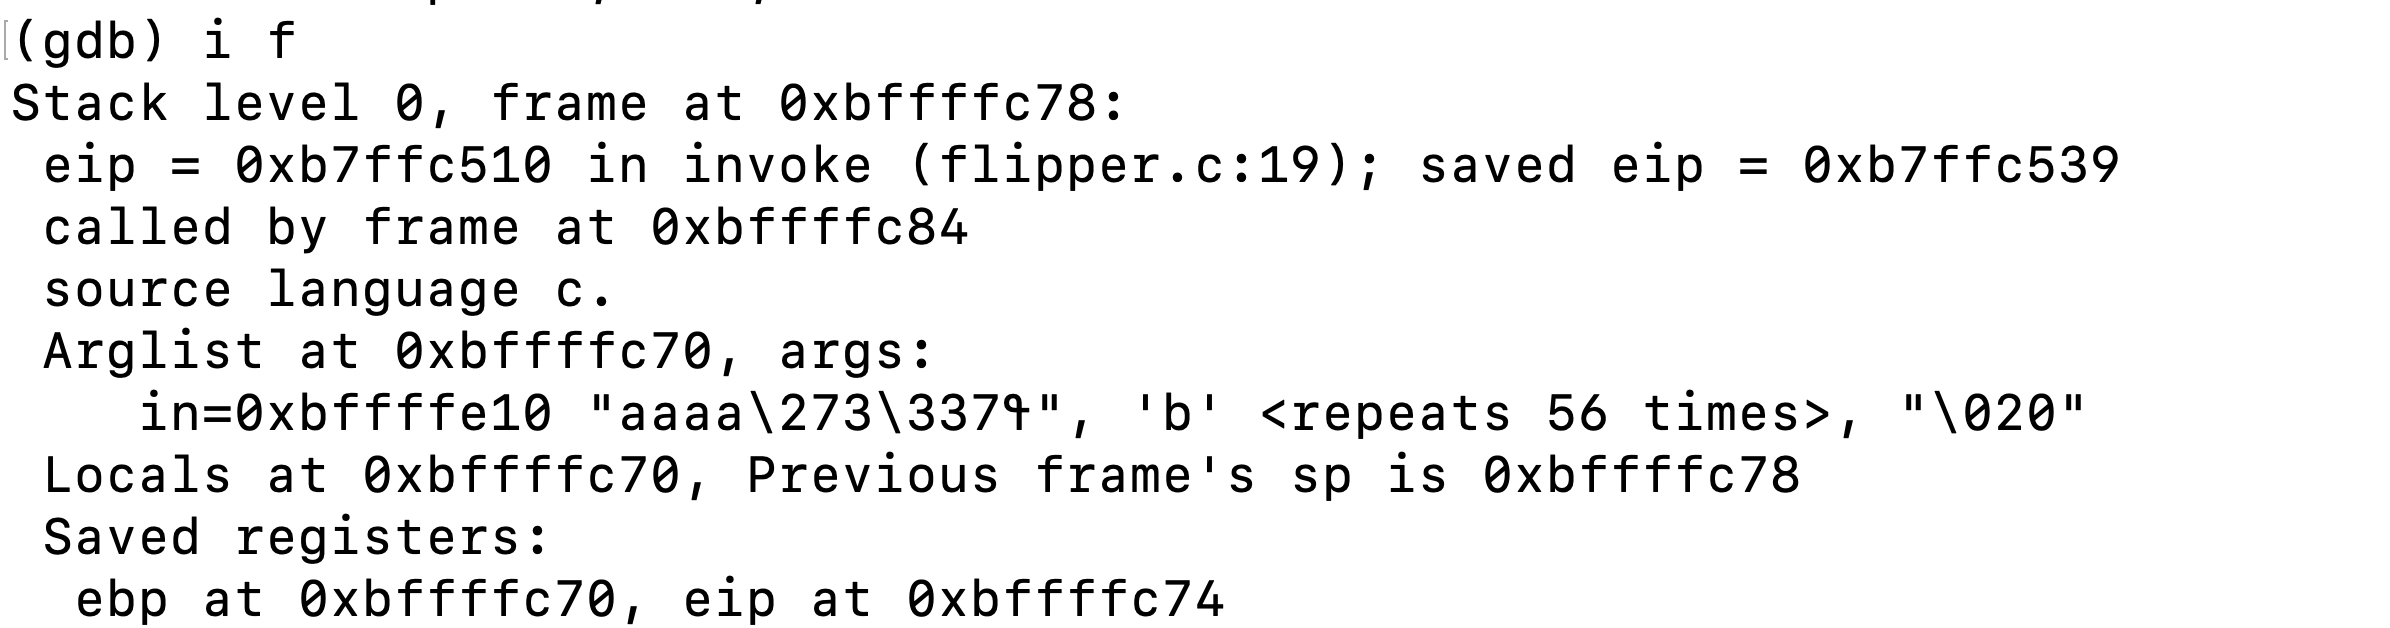
\includegraphics[width=12cm]{q4_sfp_1.png}
    \caption{address of saved \textit{ebp} (\textit{sfp}) in \textit{invoke} function}
  \end{measuredfigure}
  \label{PlP}
\end{figure}

\noindent
Next, we figure out the value of the saved \textit{ebp} (\textit{sfp}) in \textit{invoke} by using the command \textcolor{gray}{x/1x 0xbfffffc70} (i.e.\ print one byte at address \underline{0xbfffffc70}).\ Figure 21, shows that the value of the \textit{sfp} is \underline{0xbffffc7c} (we're going to want to change this value to point into the \textit{buf}).\
\newline

\begin{figure}[!htb]
  \captionsetup{singlelinecheck = false, format= hang, justification=centering, font=footnotesize, labelsep=space}
  \centering
  \begin{measuredfigure}
    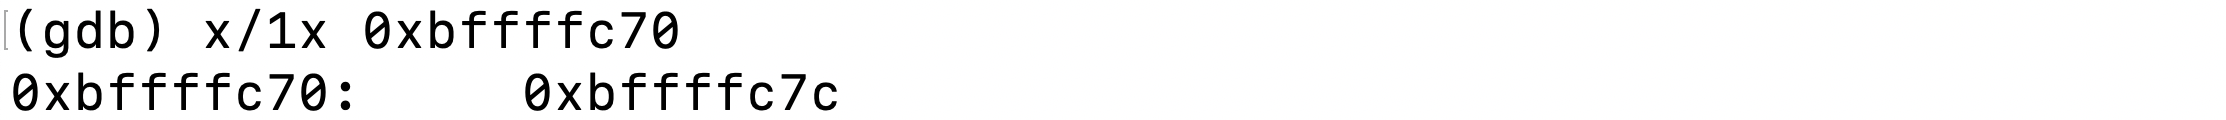
\includegraphics[width=12cm]{q4_sfp_2.png}
    \caption{value of saved \textit{ebp} (\textit{sfp}) in \textit{invoke} function}
  \end{measuredfigure}
  \label{PlP}
\end{figure}

\noindent
We then need to figure out the address of \textit{buf}, since we're going to want to alter \textit{sfp} to point into the buffer.\ To do this, we run the command \textcolor{gray}{x/17x buf} (print seventeen bytes starting at \textit{buf}) at the same break point (at \underline{line 18}).\ Figure 22, shows the address is \underline{0xbffffc30}.\ Because we can alter the least significant byte of \textit{sfp}, we will change it to \underline{0x30}.\ However, this number is xor'd on \underline{line 10} by \underline{0x20}, so we xor it by \underline{0x20} beforehand to undo this, yielding \underline{0x10}.
\newline

\begin{figure}[!htb]
  \captionsetup{singlelinecheck = false, format= hang, justification=centering, font=footnotesize, labelsep=space}
  \centering
  \begin{measuredfigure}
    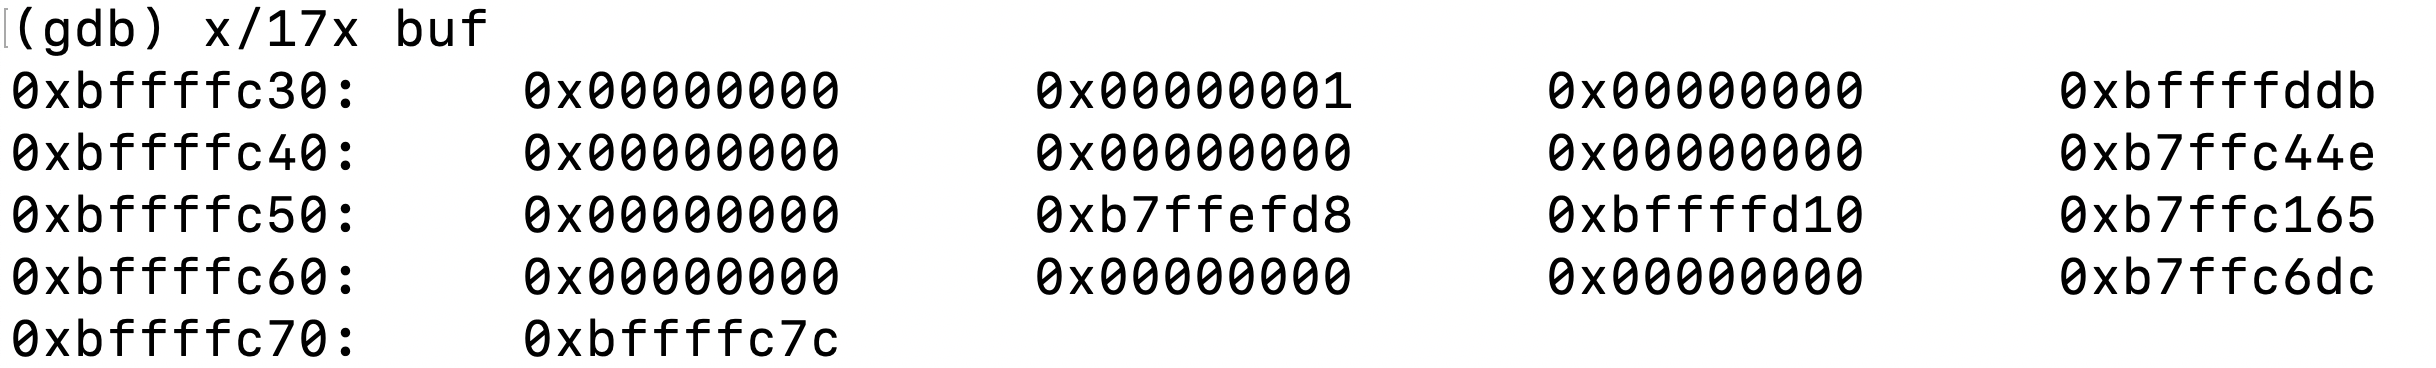
\includegraphics[width=12cm]{q4_buf.png}
    \caption{seventeen bytes starting at \textit{buf} in \textit{flip} function}
  \end{measuredfigure}
  \label{PlP}
\end{figure}

\noindent
Lastly, we need to figure out the address of our environment variable, since that will contain our shellcode.\ We use the same breakpoint at \underline{line 18} and then use the command \textcolor{gray}{x/s *((char **)environ)}, since \textit{environ} is a pointer to pointer, as it has the type \textit{char **environ} (as pointed out by user J.D.\ in stack-exchange).\ We see what looks like shell code in address \underline{0xbfffff97}.\ By executing \textcolor{gray}{x/2wx 0xbfffff97} (print two four-byte words starting at \underline{0xbfffff97}), as advised in the tips doc, we see one byte of our shellcode:\ \underline{0xcd58326a}.\ We go one byte further \textcolor{gray}{x/2wx 0xbfffff9b} and see the first two bytes of our shellcode:\ \underline{0xcd58326a} and \underline{0x89c38980}.\ Therefore, the address of the shellcode is \underline{0xbfffff9b}.\ This procedure is seen in Figure 23.\ Again, each byte in \underline{0xbfffff9b} will be xor'd on \underline{line 10} by \underline{0x20}, so we xor each byte by \underline{0x20} beforehand to undo this, yielding \underline{0x9fdfdfbb}.

\begin{figure}[!htb]
  \captionsetup{singlelinecheck = false, format= hang, justification=raggedright, font=footnotesize, labelsep=space}
  \centering
  \begin{measuredfigure}
    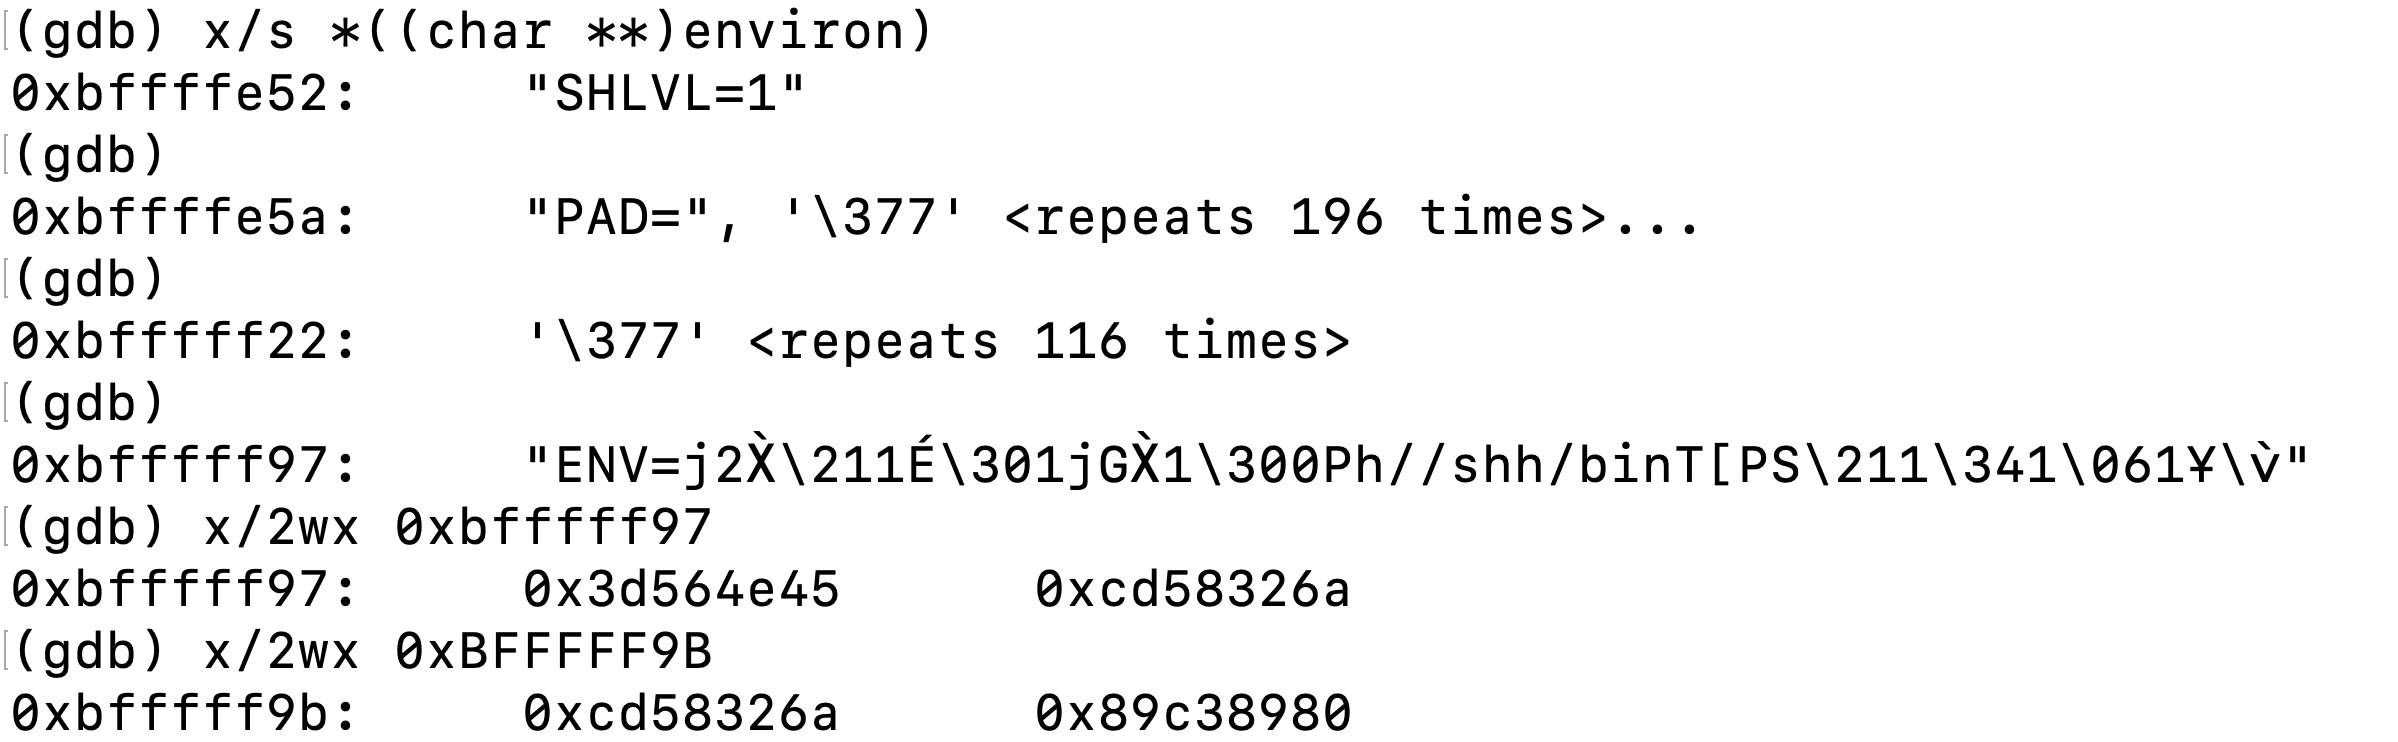
\includegraphics[width=9cm]{q4_addr_of_shellcode.png}
    \caption{determining address of shellcode in environment variable}
  \end{measuredfigure}
  \label{PlP}
\end{figure}

\subsection*{Exploit Structure}
Figure 24 highlights the stack diagram throughout the program outlined by instructor Peyrin Kao.\ Note:\ for our program, we don't set the least significant byte of \textit{sfp} to 0x00, instead we use the specific location of our buffer, i.e.\ \underline{0x30}.\ (note:\ according to instructor EvanBot on Piazza, "OSINT is accepted if source is mentioned.")

\begin{figure}[!htb]
  \captionsetup{singlelinecheck = false, format= hang, justification=centering, font=footnotesize, labelsep=space}
  \centering
  \begin{measuredfigure}
    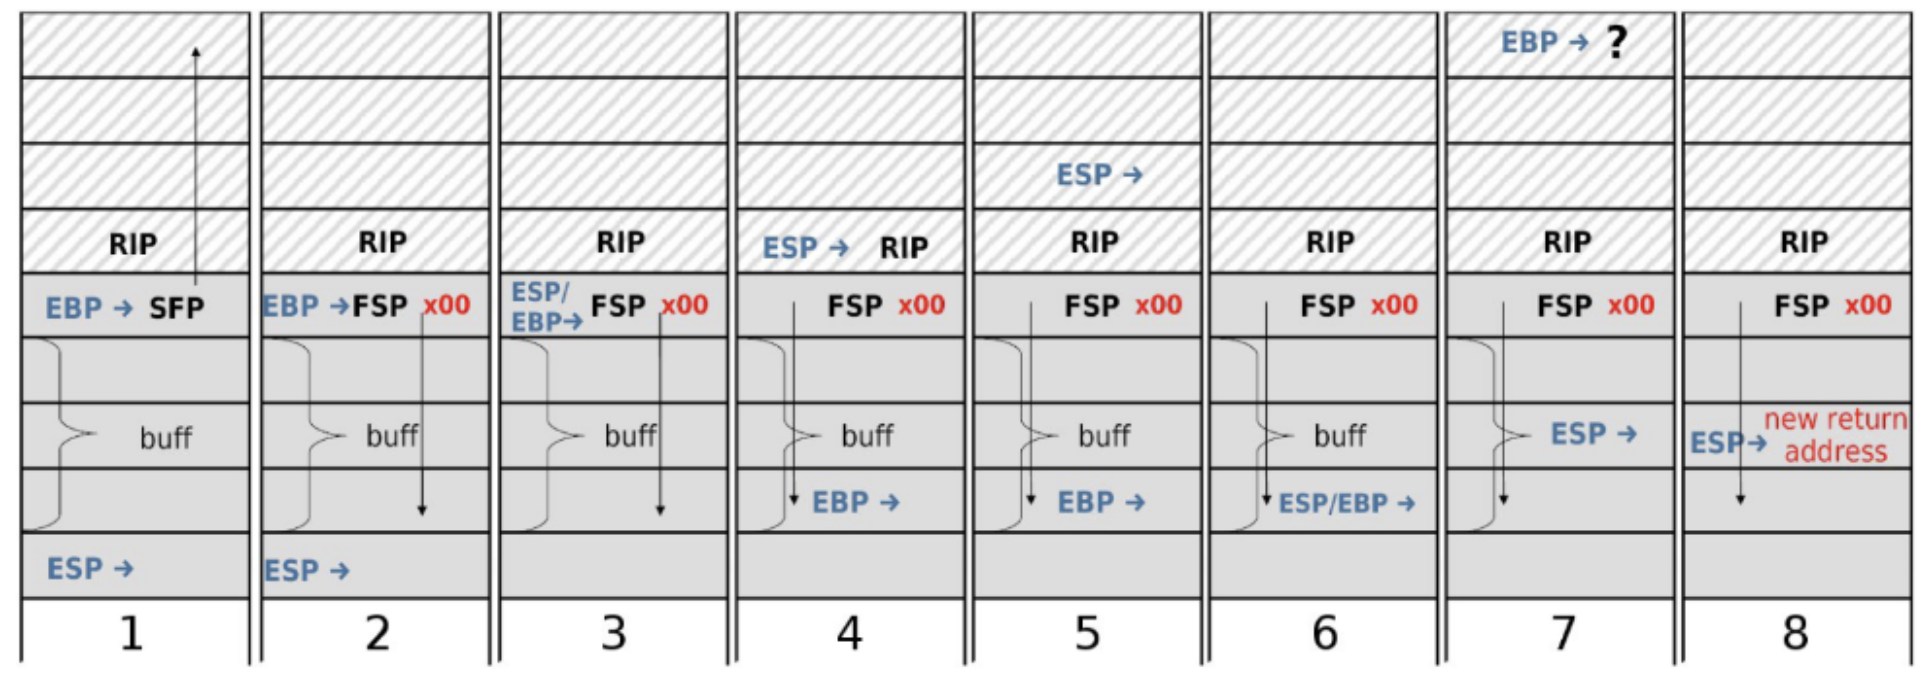
\includegraphics[width=12cm]{q4_stack_diagram.png}
    \caption{stack diagram throughout epxloit}
  \end{measuredfigure}
  \label{PlP}
\end{figure}

\noindent
The exploit has the following parts:
\begin{addmargin}[1em]{2em}
1.\ Feed \underline{4} bytes of junk into our buffer.
\newline
2.\ Feed the xor'd address of the shellcode \underline{0x9fdfdfbb} (i.e.\ each byte of \underline{0xbfffff9b} xor'd by \underline{0x20}).
\newline
3.\ Feed \underline{56} more bytes of junk to fill the rest of the buffer.
\newline
4.\ Change the least significant byte of the \textit{sfp} by feeding the last byte of the input to be \underline{0x10} (i.e.\ \underline{0x30} xor'd by \underline{0x20}), so that it points to the start of \textit{buf}.\ (note:\ we don't make it point to shellcode directly; the steps above demonstrate that \textit{fsp} should point to \underline{4} bytes below the shellcode).\
\newline
\end{addmargin}

\noindent
Consequently, as outlined in the steps, the calling function of \textit{invoke}, that is \textit{dispatch}, will eventually have its \textit{esp} pointing to the address of the shellcode and when the final step of \textcolor{gray}{pop \%eip} is executed, the \textit{eip} is overwritten with the location of the shellcode, and the shellcode will execute accordingly as the next instruction.\

\subsection*{Exploit GDB Output}
Figure 25 highlights the GDB output after inputting the  malicious exploit string.\ After \underline{4} bytes of garbage (blue), we insert the address of our shellcode \underline{0xbfffff9b} (voilet), then 56 more bytes of garbage (blue), followed by the \textit{fsp} \underline{0xbffffc30} (orange) which points to the start of \textit{buf}.

\begin{figure}[!htb]
  \captionsetup{singlelinecheck = false, format= hang, justification=centering, font=footnotesize, labelsep=space}
  \centering
  \begin{measuredfigure}
    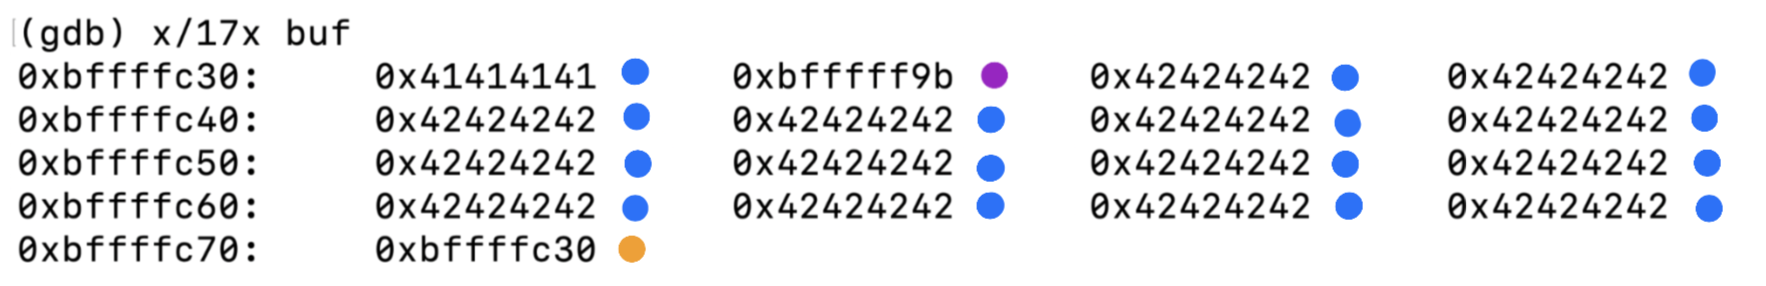
\includegraphics[width=12cm]{q4_output_1.png}
    \caption{GDB output after feeding exploit string}
  \end{measuredfigure}
  \label{PlP}
\end{figure}

\noindent
Figure 26 demonstrates, once again, that the shellcode (green) is indeed at this address (\underline{0xbfffff9b}).
\begin{figure}[!htb]
  \captionsetup{singlelinecheck = false, format= hang, justification=centering, font=footnotesize, labelsep=space}
  \centering
  \begin{measuredfigure}
    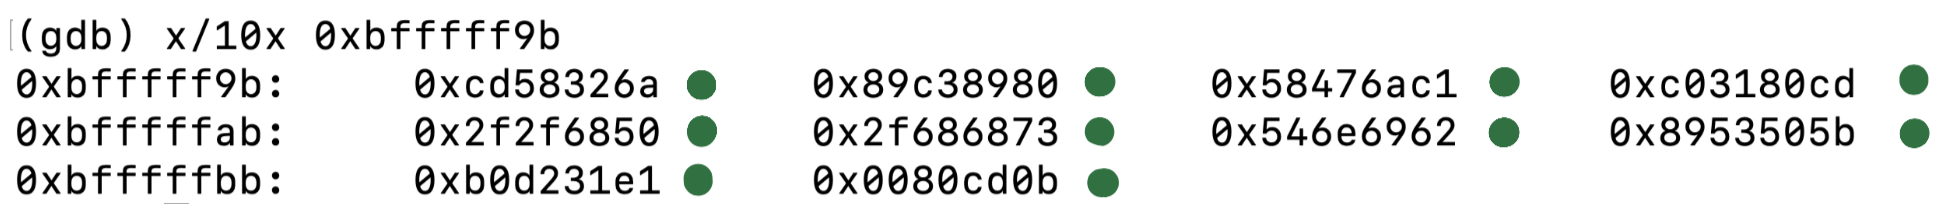
\includegraphics[width=12cm]{q4_output_2.png}
    \caption{shellcode at address 0xbfffff9b}
  \end{measuredfigure}
  \label{PlP}
\end{figure}

\subsection*{Exploit Script}
Figure 27 highlights the \textit{egg} script which provides the environment variable (shellcode) to \textit{flipper.c}.
\newline

\begin{figure}[!htb]
  \captionsetup{singlelinecheck = false, format= hang, justification=centering, font=footnotesize, labelsep=space}
  \centering
  \begin{measuredfigure}
    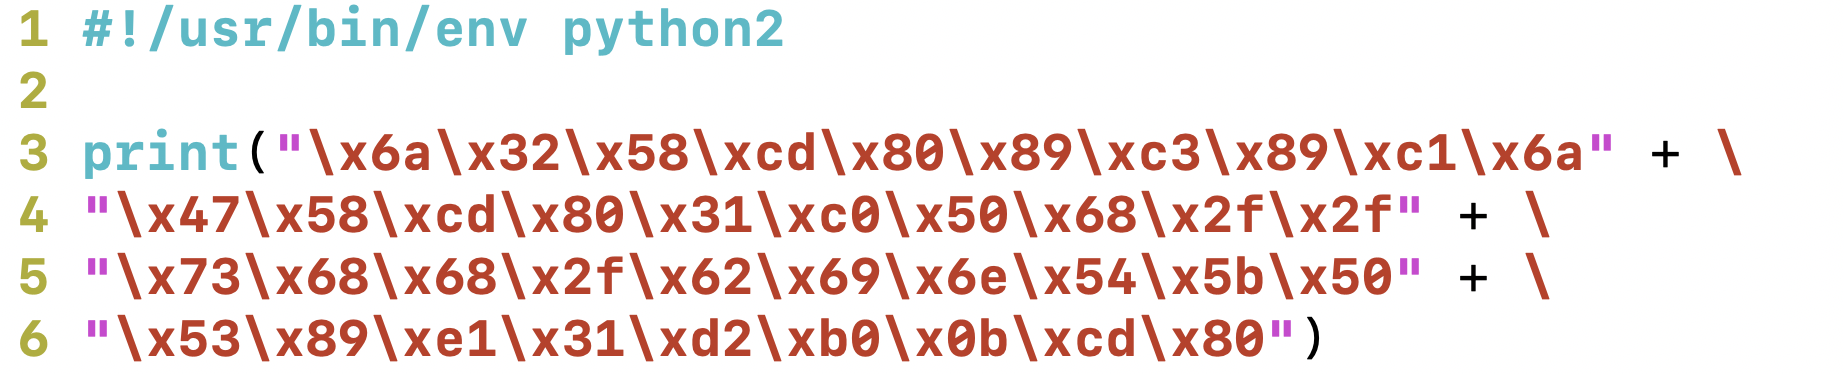
\includegraphics[width=12cm]{q4_egg.png}
    \caption{\textit{egg} script output (i.e.\ shellcode) used as env.\ variable}
  \end{measuredfigure}
  \label{PlP}
\end{figure}
\noindent
Figure 28 highlights the \textit{arg} script which provides the malicious input to exploit \textit{flipper.c}.
\begin{figure}[!htb]
  \captionsetup{singlelinecheck = false, format= hang, justification=centering, font=footnotesize, labelsep=space}
  \centering
  \begin{measuredfigure}
    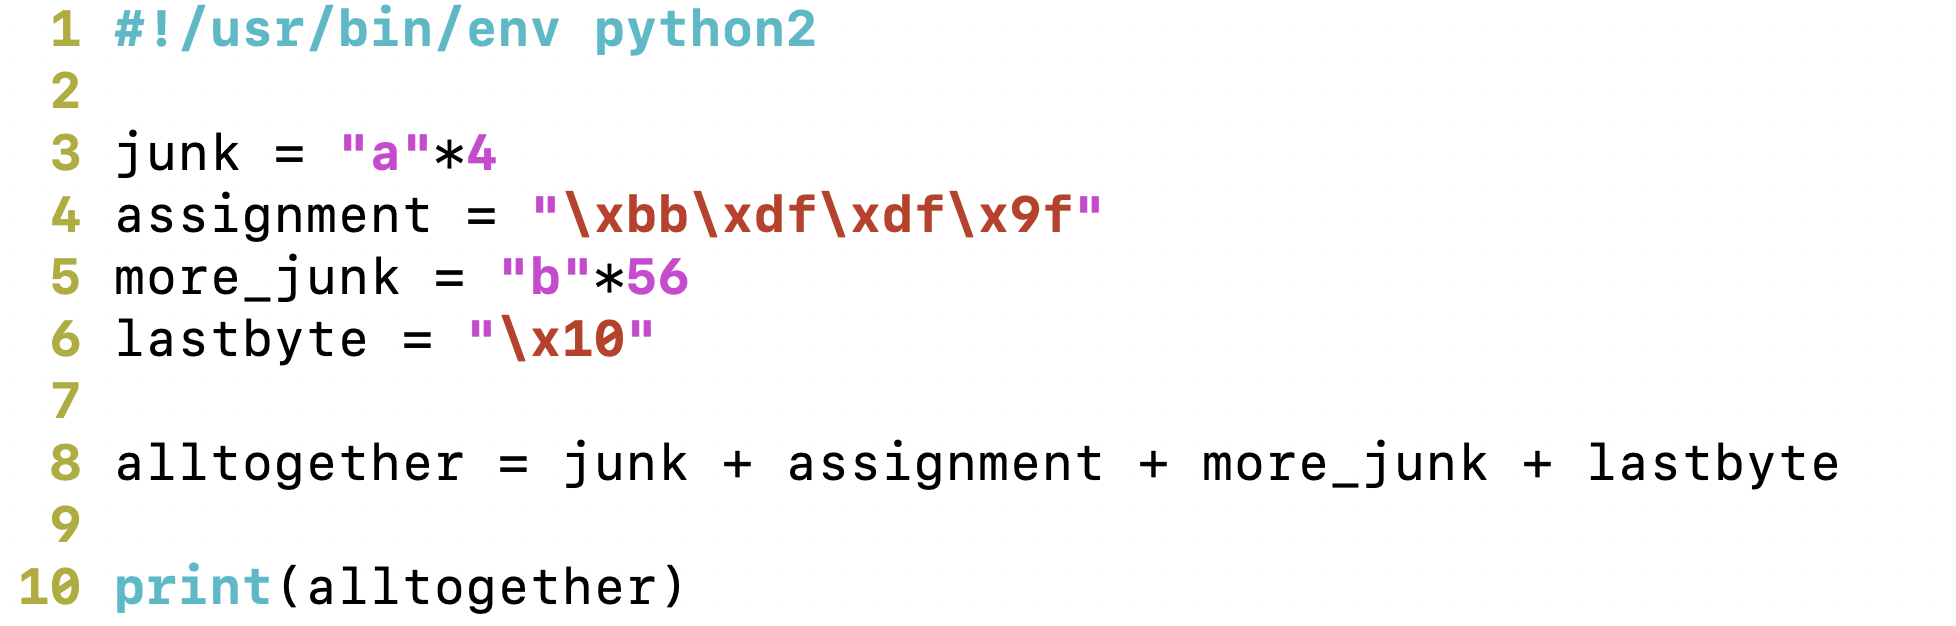
\includegraphics[width=12cm]{q4_arg.png}
    \caption{\textit{arg} script to exploit \textit{flipper.c}}
  \end{measuredfigure}
  \label{PlP}
\end{figure}



\section*{Question 5: \textit{Against the Clock}}
\subsection*{hound.c}
Figure 29 shows the code that we want to exploit, \textit{hound.c}.
\begin{figure}[!htb]
  \captionsetup{singlelinecheck = false, format= hang, justification=centering, font=footnotesize, labelsep=space}
  \centering
  \begin{measuredfigure}
    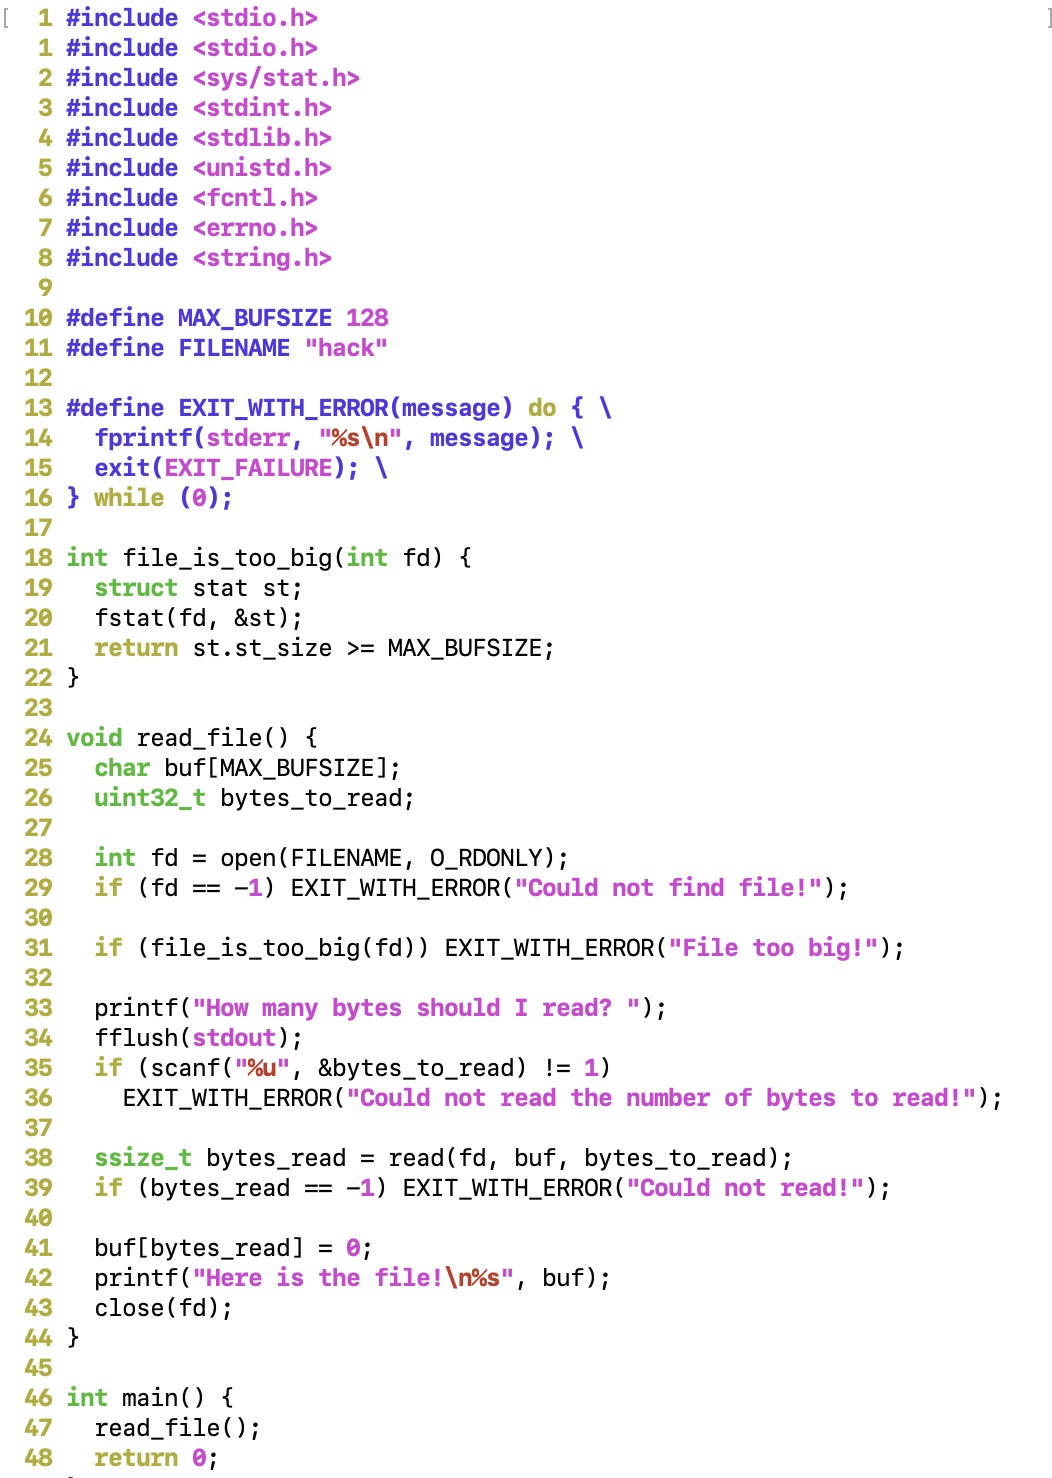
\includegraphics[width=12cm]{q5_hound.c.png}
    \caption{\textit{hound.c} source code}
  \end{measuredfigure}
  \label{PlP}
\end{figure}

\subsection*{Main Idea}
TL;DR:\ This program is an example of the classic \textbf{time-of-check to time-of-use} exploit.\ The program checks the size of the file at \underline{line 31} but then the file is not read till \underline{line 38}.\ Through some evil engineering, one can open the file and change the contents (and therefore size) after the check and before the read.\ Consequently, one can then \textbf{overflow} the buffer by making the file's contents larger than \textit{MAX\_BUFSIZE}.
\newline

\noindent
To exploit the code, one has to first feed in a file that will bypass \underline{line 31}.\ Any file that has contents less than \textit{MAX\_BUFSIZE} should suffice.\ Then, one could run the program and then try to immediately change the file in the hope that it happens after \underline{line 31} and before \underline{line 38}; however, this causes a race condition (it could work, it could not).\ Instead, we notice that on \underline{line 33} there is \textit{printf} to the user asking for the number of bytes and \textit{scanf} on \underline{line 35} to read in the user's response from stdin.\ One can use \textit{recv} to receive the message from \textit{printf}, and then while \textit{scanf} is waiting for the response, change the contents of the file to be larger than \textit{MAX\_BUFSIZE}.\ After, one can finally respond to the \textit{scanf} by inputting the size of the edited file, and then finally, the buffer will be overflown in \textit{read} on \underline{line 38}.
\newline

\noindent
Specifically, we fill the buffer with anything that makes us happy (i.e.\ junk), then overwrite the saved return address on the stack (\textit{rip}) with the address of the shellcode (we'll choose the byte directly after), and insert the shellcode above the \textit{rip} accordingly.\

\subsection*{Magic Numbers}
First, we determine the address of the buffer, \textit{buf}.\ To do this, we open up GDB and place a break at \underline{line 27}, \textcolor{gray}{b 27}.\ By running the program, hitting the break, and then using the command \textcolor{gray}{x/16x buf}, we determine the address of the buffer:\ \underline{0xbffffc48}, seen in Figure 30.\
\newline

\begin{figure}[!htb]
  \captionsetup{singlelinecheck = false, format= hang, justification=centering, font=footnotesize, labelsep=space}
  \centering
  \begin{measuredfigure}
    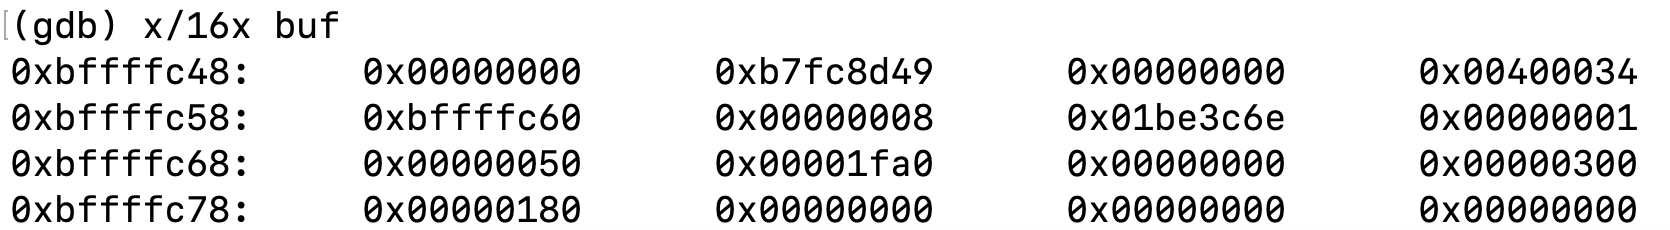
\includegraphics[width=12cm]{q5_magic_numbers_2.png}
    \caption{sixteen bytes starting at \textit{buf} in \textit{read\_file} function}
  \end{measuredfigure}
    \label{PlP}
\end{figure}

\noindent
Next, we determine the location of the saved \textit{eip} (\textit{rip}) for the function we want to exploit, \textit{read\_file}.\ By using the break statement on \underline{line 27} and the command \textcolor{gray}{i f}, we see \textit{eip} was stored at address \underline{0xbfffcdc}, shown in\ Figure 31.
\newline

\begin{figure}[!htb]
  \captionsetup{singlelinecheck = false, format= hang, justification=centering, font=footnotesize, labelsep=space}
  \centering
  \begin{measuredfigure}
    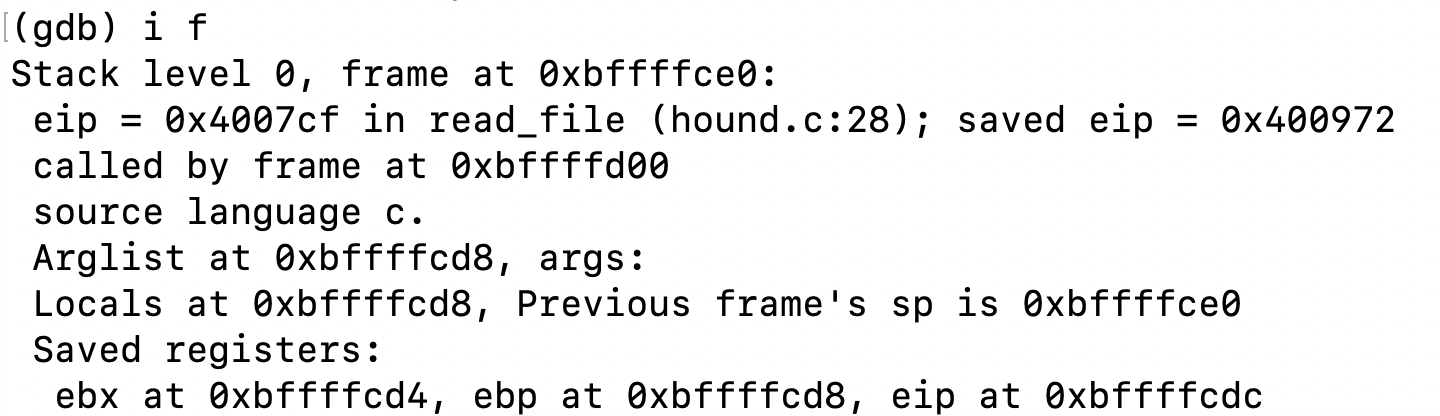
\includegraphics[width=12cm]{q5_magic_numbers_1.png}
    \caption{address of saved \textit{eip} (\textit{rip}) in \textit{read\_file} function}
  \end{measuredfigure}
    \label{PlP}
\end{figure}

\noindent
By doing so, we learned that the location of the return address from this function is
\underline{148} bytes away from the start of the buffer \textit{buf} (\underline{0xbffffcdc $-$ 0xbffffc48 $=$ 0x94 $=$ 148}).
\subsection*{Exploit Structure}
Figure 32 paints the stack diagram before the exploit.
\begin{figure}[!htb]
  \captionsetup{singlelinecheck = false, format= hang, justification=centering, font=footnotesize, labelsep=space}
  \centering
  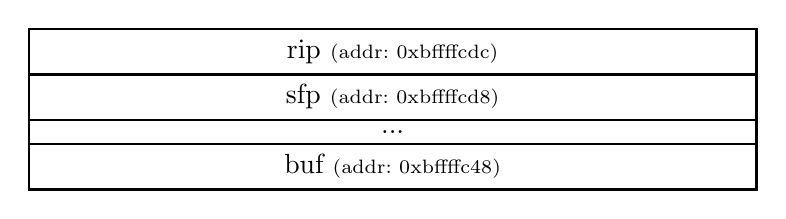
\begin{tikzpicture}[stack/.style={rectangle split, rectangle split parts=#1,draw, anchor=center}]
  \node[stack=4, line width=1pt, text width=9cm, text centered]  {
  \nodepart{one}rip \scriptsize(addr:\ 0xbffffcdc)
  \nodepart{two}sfp \scriptsize(addr:\ 0xbffffcd8)
  \nodepart{three}...
  \nodepart{four}buf \scriptsize(addr:\ 0xbffffc48)
  };
  \end{tikzpicture}
  \caption{stack diagram before exploit}
  \label{PlP}
\end{figure}

\noindent
Part one (getting past file-size check on \underline{line 31}):
\begin{addmargin}[1em]{2em}
1.\ To exploit the code, one has to first feed in a file that will bypass \underline{line 31}.\ Any file that has contents less than \textit{MAX\_BUFSIZE} should suffice.
\end{addmargin}
Part two (changing the file \& overflowing buffer).\
\begin{addmargin}[1em]{2em}
1.\ Use \textit{recv} to intercept the message from \textit{printf}.\ \textit{recv} acts like a break point in that it stalls until first print statement.\ Thus, any code in our exploit after \textit{recv} will be sure to execute after the \textit{printf} statement on \underline{line 33} (as desired).\ Furthermore, \textit{recv} needs us to specify the number of bytes to intercept.\ So long as it is less than the number of bytes in the message from \textit{printf} (e.g.\ 5), it should work.\ Otherwise, it will wait until it reads that many bytes.
\newline
\noindent
2.\ Next, we run our code to change our file.\ Since there is a \textit{scanf} on \underline{line 35}, the program has effectively paused until the user input is sent.\ Therefore, our code will run before \underline{line 36} (as desired).\ Here we open the file, and feed the following input:
\begin{addmargin}[1em]{2em}
a)\ Feed \underline{148} bytes of junk to overwrite the buffer, everything in-between, and the \textit{sfp}.
\newline
\noindent
b)\ Overwrite the \textit{rip} with the address of the shellcode.\ Since we are putting the shellcode directly after the \textit{rip}, we overwrite the \textit{rip} with \underline{0xbfffce0} (\underline{0xbfffcdc + 4}).\
\newline
\noindent
c)\ Finally, insert the shellcode directly after the \textit{rip}.\
\end{addmargin}
3.\ Finally, respond to the \textit{scanf} by sending the number of bytes of the changed file.
\newline
\end{addmargin}

\begin{figure}[!htb]
  \captionsetup{singlelinecheck = false, format= hang, justification=centering, font=footnotesize, labelsep=space}
  \centering
  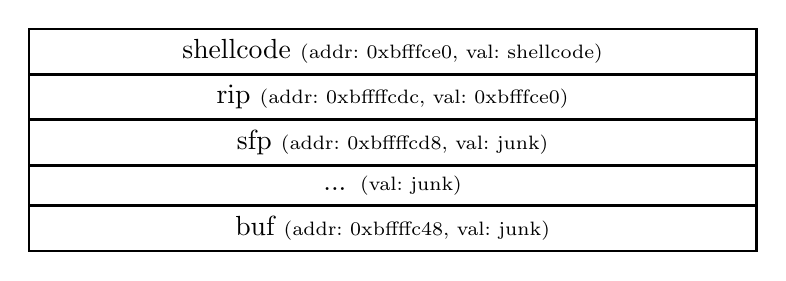
\begin{tikzpicture}[stack/.style={rectangle split, rectangle split parts=#1,draw, anchor=center}]
  \node[stack=5, line width=1pt, text width=9cm, text centered]  {
  \nodepart{one}shellcode \scriptsize(addr:\ 0xbfffce0, val:\ shellcode)
  \nodepart{two}rip \scriptsize(addr:\ 0xbffffcdc, val:\ 0xbfffce0)
  \nodepart{three}sfp \scriptsize(addr:\ 0xbffffcd8, val:\ junk)
  \nodepart{four}... \scriptsize(val:\ junk)
  \nodepart{five}buf \scriptsize(addr:\ 0xbffffc48, val:\ junk)
  };
  \end{tikzpicture}
  \caption{stack diagram after buffer overflow}
  \label{PlP}
\end{figure}

\noindent
Figure 33 reflects the stack diagram once the input of the exploit is fed in.\ This causes the \textit{read\_file} function to execute the shellcode at address \underline{0xbfffce0} upon return.

\subsection*{Exploit GDB Output}
Figure 34 highlights the GDB Output after feeding malicious input.\ After \underline{148} bytes of garbage (blue), the \textit{rip} (red) is overwritten with \underline{0xbffffcd0}, which points to the shellcode (green), which is directly after the \textit{rip}.\

\begin{figure}[!htb]
  \captionsetup{singlelinecheck = false, format= hang, justification=centering, font=footnotesize, labelsep=space}
  \centering
  \begin{measuredfigure}
    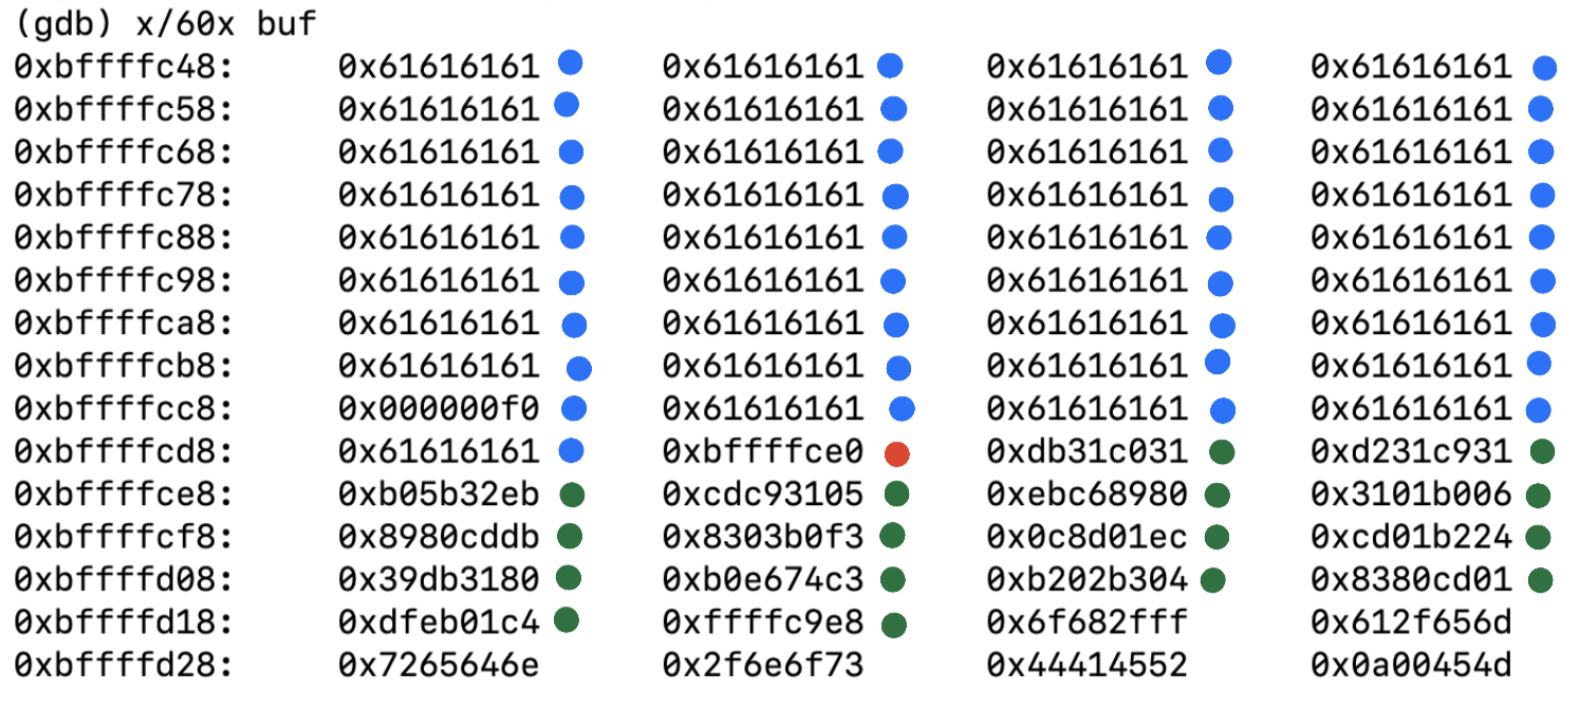
\includegraphics[width=12cm]{q5_gdb_output.png}
    \caption{GDB output after feeding exploit string}
  \end{measuredfigure}
    \label{PlP}
\end{figure}

\noindent
\subsection*{Exploit Script}
Figure 35 highlights the \textit{interact} script, which executes the exploit of \textit{hound.c}.
\begin{figure}[!htb]
  \captionsetup{singlelinecheck = false, format= hang, justification=centering, font=footnotesize, labelsep=space}
  \centering
  \begin{measuredfigure}
    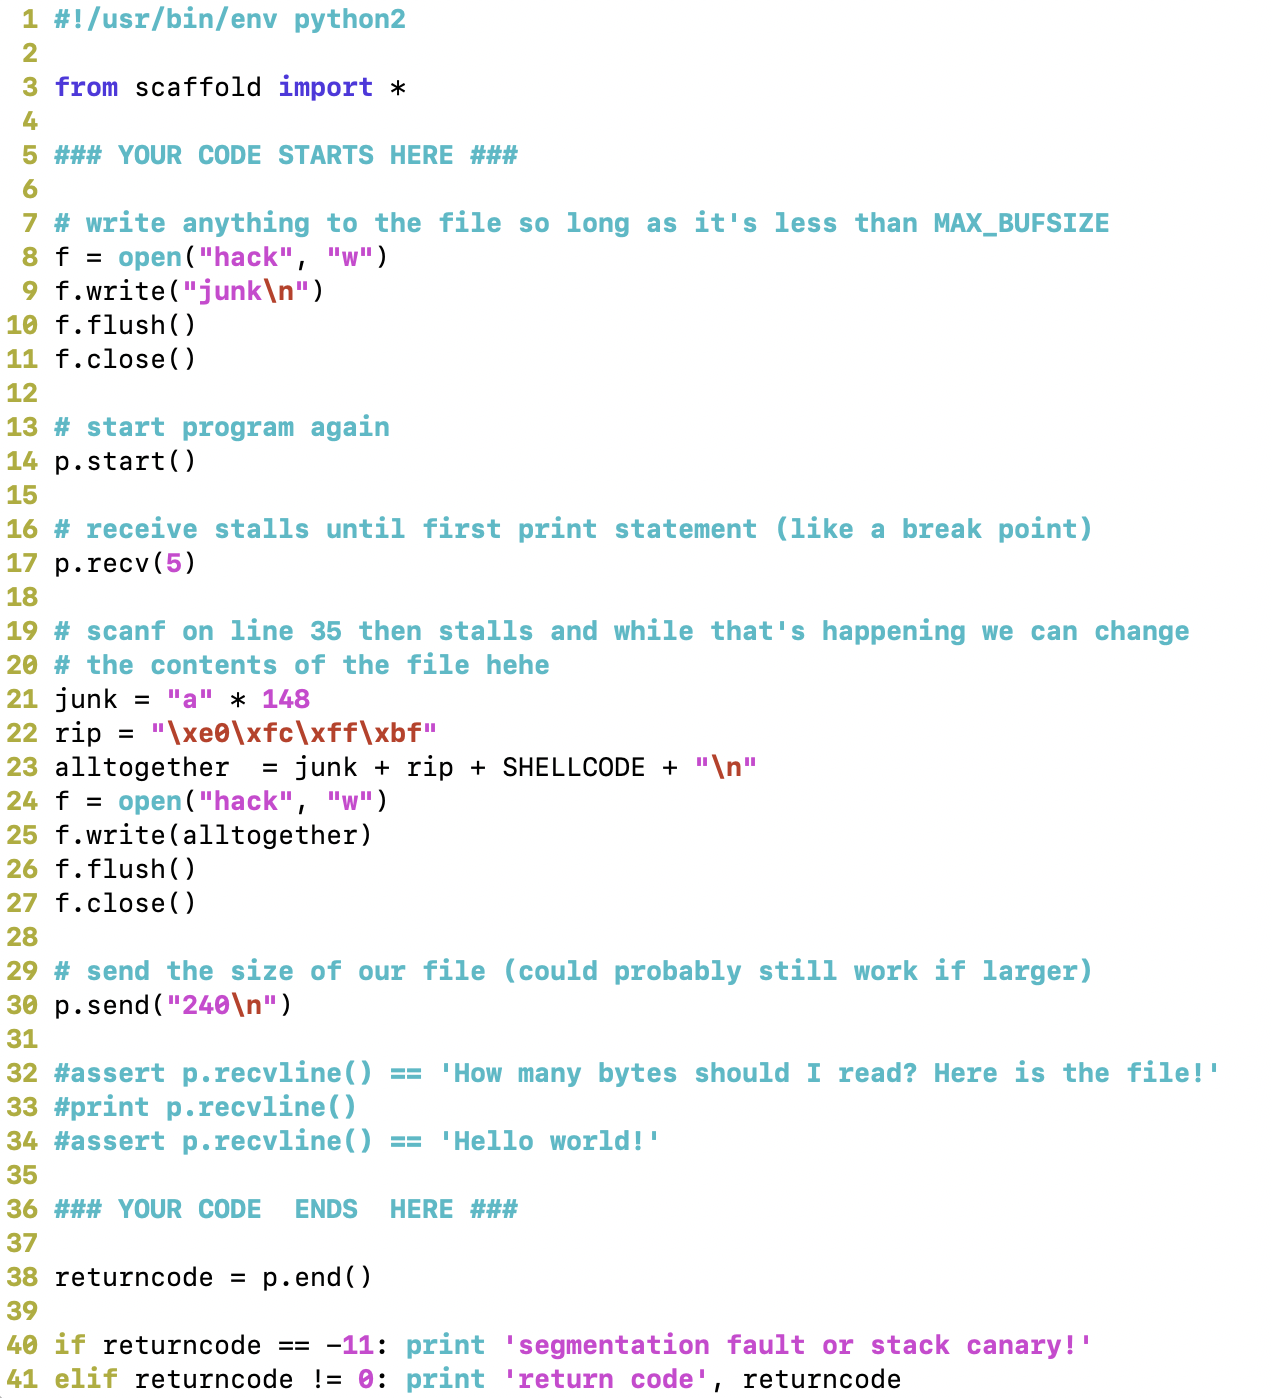
\includegraphics[width=9cm]{q5_interact.png}
    \caption{\textit{interact} script to exploit hound.c}
  \end{measuredfigure}
  \label{PlP}
\end{figure}
\section*{Question 6: \textit{The Last Bastion}}
\subsection*{uplink.c}
Figure 36 shows the code that we want to exploit, \textit{uplink.c}.
\begin{figure}[!htb]
  \captionsetup{singlelinecheck = false, format= hang, justification=centering, font=footnotesize, labelsep=space}
  \centering
  \begin{measuredfigure}
    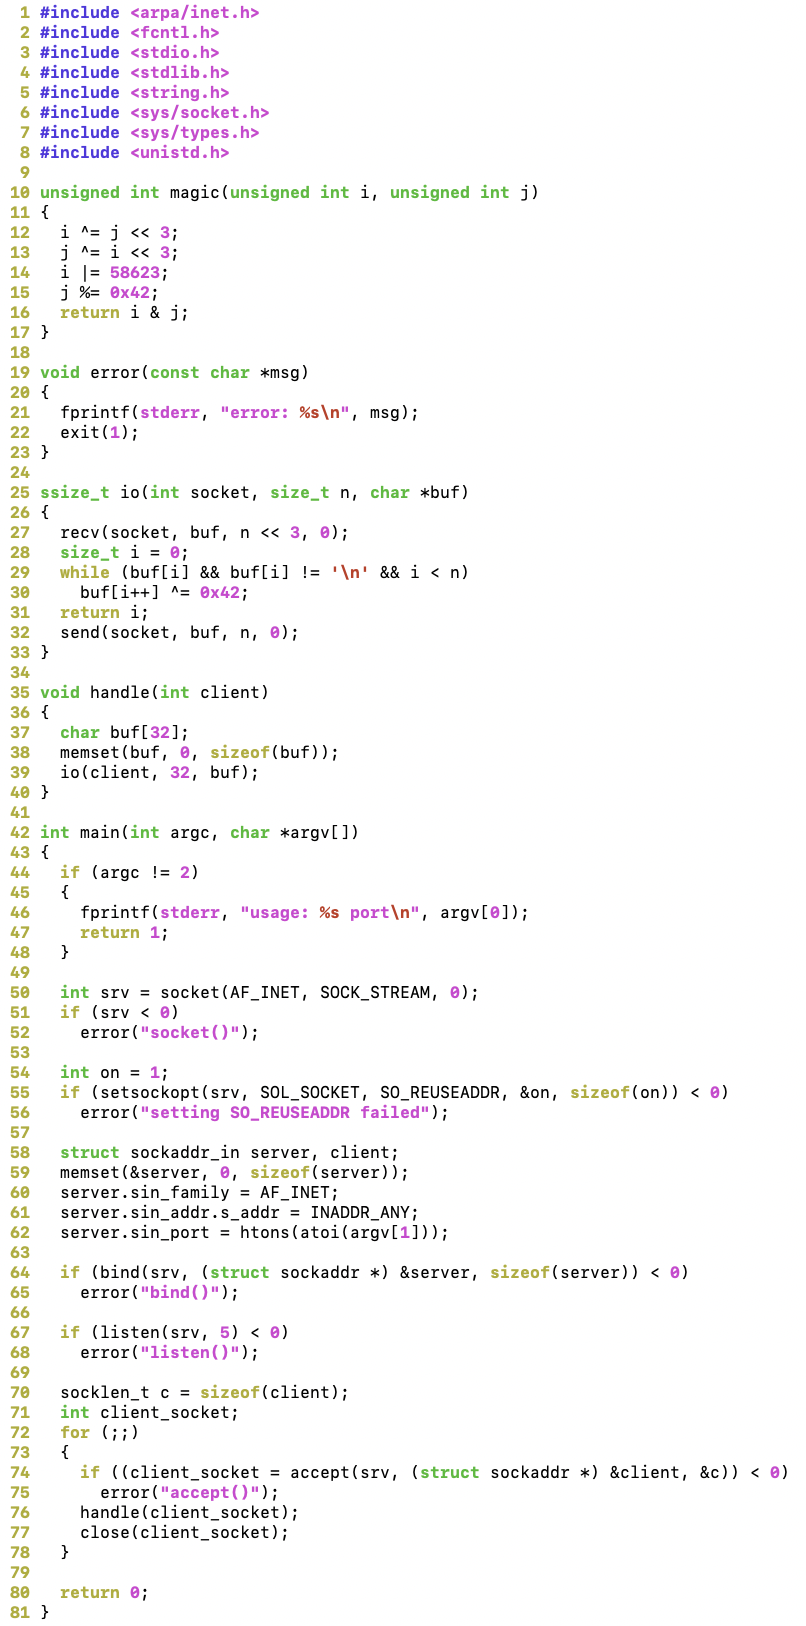
\includegraphics[width=8cm]{q6_uplink.c.png}
    \caption{\textit{uplink.c} source code}
  \end{measuredfigure}
  \label{PlP}
\end{figure}

\subsection*{Main Idea}
TL;DR:\ This is an example of a \textbf{ret2esp} exploit.\ Since \textbf{ASLR} is enabled, our \textit{rip} will not always be at the same location, and therefore, we cannot overwrite it with a known address.\ We therefore, take advantage of the fact that the code has the following instruction:\ \textcolor{gray}{jmp *esp}.\ When we \textbf{overflow} the buffer, we overwrite \textit{rip} (whose relative location from the buffer we can determine) with this instruction, and put the shellcode at the previous frame's stack pointer (whose relative address we can also determine).
\newline

\noindent
Even though we can overflow the buffer on \underline{line 27}, we can't perform our normal exploit process because of \textbf{ASLR}.\ That is, \textit{rip} will not always be at the same location, and therefore, we cannot overwrite it with a known address.\ However, we can take advantage of \underline{line 14} which has the \textcolor{gray}{jmp *esp} instruction.\ When we \textbf{overflow} the buffer, we overwrite \textit{rip} (whose relative location we know by subtracting the location of the saved \textit{eip} (\textit{rip}) by the location of \textit{buf}) with this instruction.\ Furthermore, we know that the last part of the epilogue is \textcolor{gray}{pop \%eip}.\ When this happens in \textit{handle}:\ 1) \textit{eip} will point to \textcolor{gray}{jmp *esp}, i.e.\ this is the next instruction to execute, and after this instruction executes, 2) \textit{esp} will point to the top of the previous frame (whose relative location we know by subtracting its distance from \textit{buf}), which is where we'll place our shellcode.


\subsection*{Magic Numbers}
Since \textbf{ASLR} is enabled, we cannot determine the absolute address of the saved \textit{eip} (\textit{rip}) in the \textit{handle} function.\ Instead, we can figure out the relative distance from \textit{buf} to the saved \textit{eip} (\textit{rip}).\
\newline

\noindent
First, we determine the address of the buffer, \textit{buf}.\ To do this, we open up GDB and place a break at \underline{line 37}, \textcolor{gray}{b 37}.\ By running the program, hitting the break, and then using the command \textcolor{gray}{x/16x buf}, we determine the address of the buffer:\ \underline{0xbfd98a20}, seen in Figure 37.\

\begin{figure}[!htb]
  \captionsetup{singlelinecheck = false, format= hang, justification=centering, font=footnotesize, labelsep=space}
  \centering
  \begin{measuredfigure}
    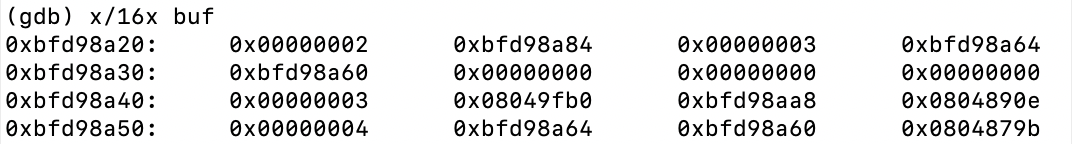
\includegraphics[width=11cm]{q6_magic_numbers_1.png}
    \caption{sixteen bytes starting at \textit{buf} in \textit{handle} function}
  \end{measuredfigure}
  \label{PlP}
\end{figure}

\noindent
Next, we determine the location of the saved \textit{eip} (\textit{rip}) for the function we want to exploit, \textit{handle}.\ By using the break statement on \underline{line 37} and the command \textcolor{gray}{i f}, we see \textit{eip} was stored at address \underline{0xbfd98a4c}, shown in\ Figure 38.
\newline

\noindent
By doing so, we learned that the location of the return address from this function is
\underline{44} bytes away from the start of \textit{buf} (\underline{0xbfd98a4c} $-$ \underline{0xbfd98a20} $=$ \underline{0x2c} $=$ \underline{44}).
\newline

\begin{figure}[!htb]
  \captionsetup{singlelinecheck = false, format= hang, justification=raggedright, font=footnotesize, labelsep=space}
  \centering
  \begin{measuredfigure}
    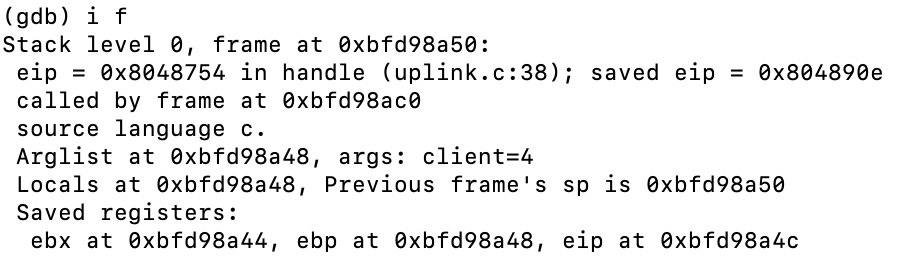
\includegraphics[width=10cm]{q6_magic_numbers_2.png}
    \caption{address of saved \textit{eip} (\textit{rip}) in \textit{handle} function and previous frame's stack pointer}
  \end{measuredfigure}
  \label{PlP}
\end{figure}

\noindent
Additionally, we need to figure out the relative distance from \textit{buf} to the previous frames stack pointer, since this is where we'll insert our shellcode.\ Figure 38 reveals that the previous frame's stack pointer is at address \underline{0xbfd98a50}.\ Therefore, we deduce it is the byte directly after \textit{rip} and is \underline{48} bytes away from the start of \textit{buf} (\underline{0xbfd98a50 $-$ 0xbfd98a20 $=$ 0x30 $=$ 48}).
\newline

\noindent
Next, we determine the location of the \textcolor{gray}{jmp *esp} instruction.\ Section 8.3 of \textit{ASLR Smack \& Laugh Reference} by Tilo M\"uller suggests to use the command \textcolor{gray}{dissas \textit{function\_name}} to see the assembly output of function\_name.\ We know that hex \underline{0xffe4} corresponds to \textcolor{gray}{jmp *esp}, so we look for that.\ By executing the command \textcolor{gray}{dissas magic} in GDB, we see the instruction \textcolor{gray}{orl \$0xe4ff, 0x8(\%ebp)} at address \underline{0x08048663}, in Figure 39, which is the hex that we're looking for (\underline{0xffe4} is interpreted as \textcolor{gray}{jmp *esp}).

\begin{figure}[!htb]
  \captionsetup{singlelinecheck = false, format= hang, justification=centering, font=footnotesize, labelsep=space}
  \centering
  \begin{measuredfigure}
    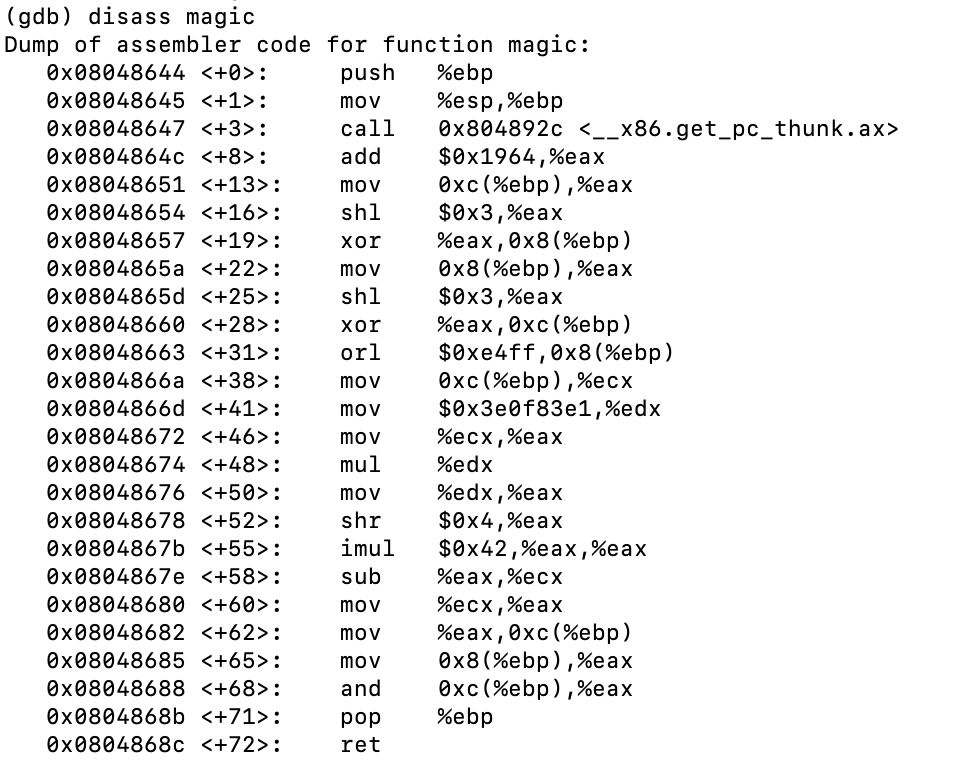
\includegraphics[width=12cm]{q6_disass_magic.png}
    \caption{assembly instructions corresponding to \textit{magic} function}
  \end{measuredfigure}
  \label{PlP}
\end{figure}

\noindent
Finally, one needs to go \underline{3} bytes past this instruction to skip the original \textcolor{gray}{orl} instruction.\ After doing so, one can see the desired instruction, \textcolor{gray}{jmp *esp}, at address \underline{0x8048666} (\underline{0x08048663} + 3), in Figure 40.

\begin{figure}[!htb]
  \captionsetup{singlelinecheck = false, format= hang, justification=centering, font=footnotesize, labelsep=space}
  \centering
  \begin{measuredfigure}
    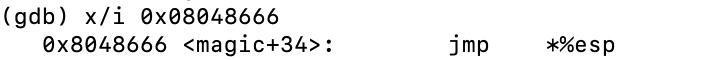
\includegraphics[width=12cm]{q6_jump_esp.png}
    \caption{location of \textit{jump *esp} instruction}
  \end{measuredfigure}
  \label{PlP}
\end{figure}

\subsection*{Exploit Structure}
The stack diagram can be see in Figure 41, as diligently illustrated by Tyler Muller.\ (note:\ according to instructor EvanBot on Piazza, "OSINT is accepted if source is mentioned.")
\newline

\begin{figure}[!htb]
  \captionsetup{singlelinecheck = false, format= hang, justification=centering, font=footnotesize, labelsep=space}
  \centering
  \begin{measuredfigure}
    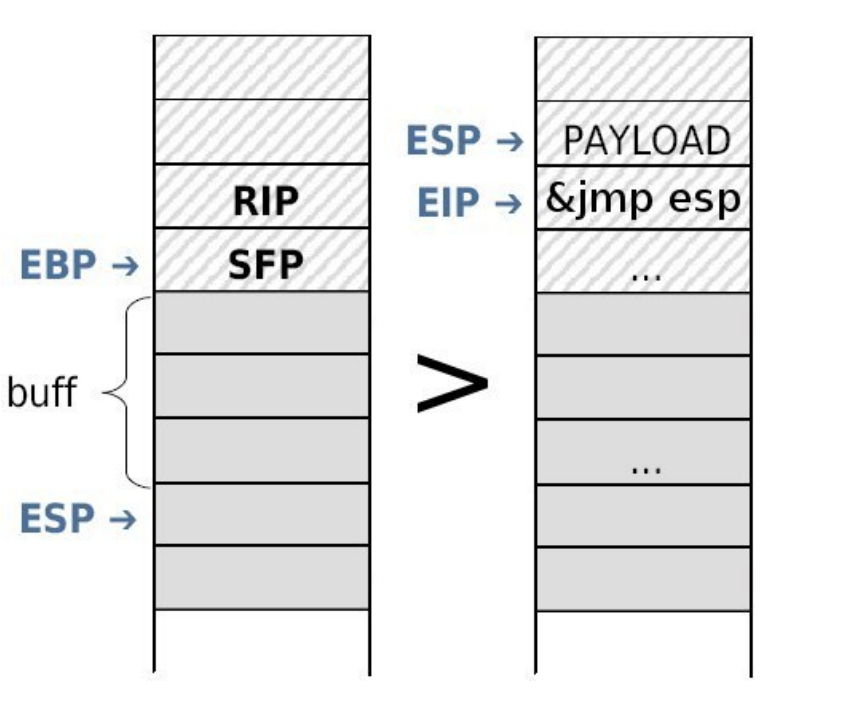
\includegraphics[width=9cm]{q6_stack_diagram.png}
    \caption{stack diagram before and after exploit}
  \end{measuredfigure}
  \label{PlP}
\end{figure}

\noindent
The exploit has three parts:
\begin{addmargin}[1em]{2em}
1.\ Feed in \underline{44} bytes of garbage since we know that the buffer is \underline{44} bytes away from \textit{rip}.
\newline
\noindent
2.\ Overwrite \textit{rip} with the address \underline{0x8048666}, i.e.\ address of \textcolor{gray}{jmp *esp} instruction.
\newline
\noindent
3.\ Place shellcode directly after \textit{rip} since we deduced in Magic Numbers that's where esp will point to after \textcolor{gray}{pop \%eip} in \textit{handle}.
\newline
\end{addmargin}
\noindent
This causes \textit{handle} to execute the instructions at \underline{0x8048666} (\textcolor{gray}{jmp *esp}) upon return.\ Which consequently jumps to \textit{esp}, which at this point is the shellcode.

\subsection*{Exploit GDB Output}
To get the GDB output, we set a break point at \underline{line 27} (\textcolor{gray}{b 27}) and use a separate terminal to feed the exploit string (\textcolor{gray}{./debug-exploit}).\ Once that is done, the program moves on to the next line, and we can see the contents of our buffer (\textcolor{gray}{x/35x buf}, i.e.\ print 35 bytes starting at \textit{buf}).
\begin{figure}[!htb]
  \captionsetup{singlelinecheck = false, format= hang, justification=centering, font=footnotesize, labelsep=space}
  \centering
  \begin{measuredfigure}
    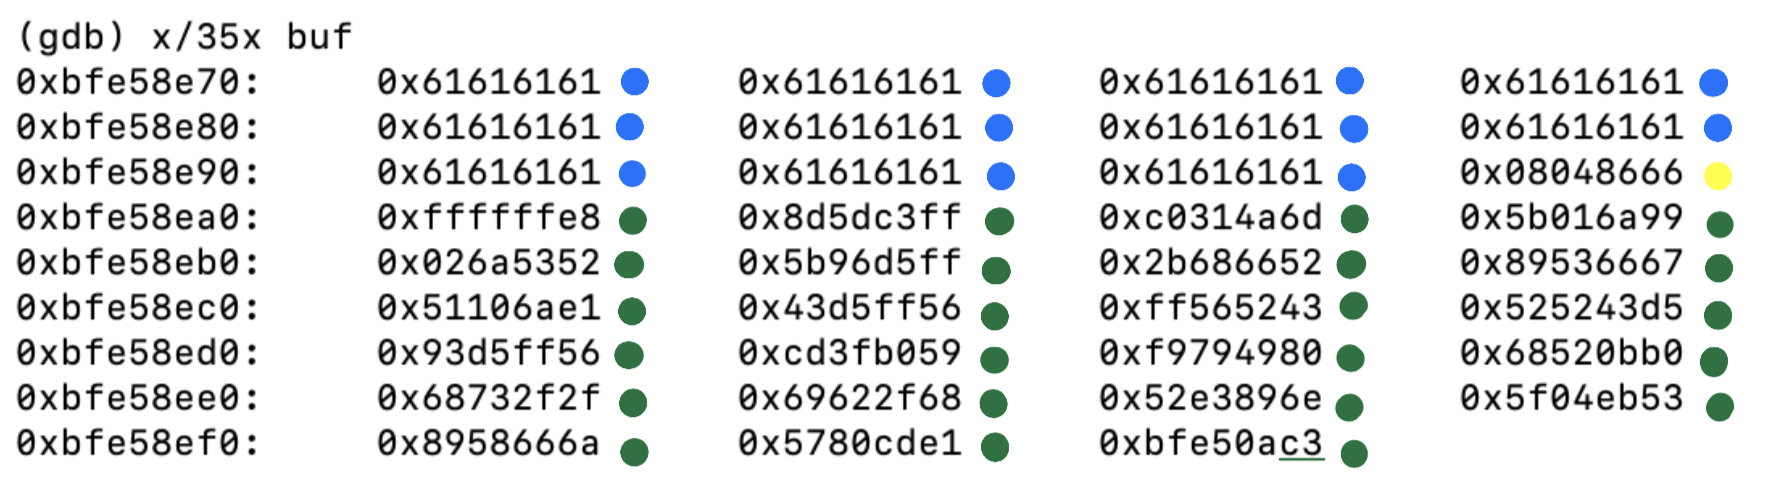
\includegraphics[width=12cm]{q6_gdb_output_1.png}
    \caption{GDB output after feeding exploit string}
  \end{measuredfigure}
    \label{PlP}
\end{figure}
\newline

\noindent
Figure 42 highlights the contents of our buffer after doing so.\ After \underline{44} bytes of garbage (blue), the \textit{rip} is overwritten with the address of the \textcolor{gray}{jmp *esp} instruction \underline{0x08048666} (yellow), which, after executed, will jump to \textit{esp} (the byte after \textit{rip}) which is where our shellcode (green) is.

\subsection*{Exploit Script}
Figure 43 highlights the \textit{egg} script, which provides the malicious input to exploit \textit{uplink.c}.
\begin{figure}[!htb]
  \captionsetup{singlelinecheck = false, format= hang, justification=centering, font=footnotesize, labelsep=space}
  \centering
  \begin{measuredfigure}
    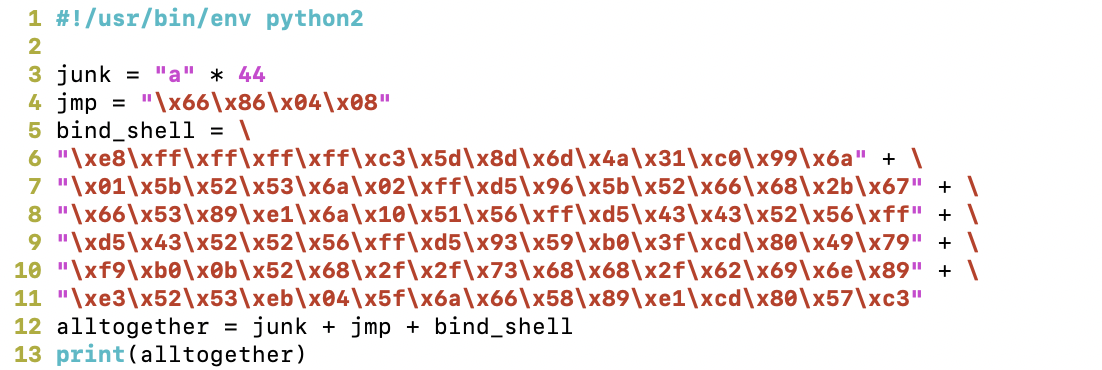
\includegraphics[width=12cm]{q6_egg.png}
    \caption{\textit{egg} script to exploit \textit{uplink.c}}
  \end{measuredfigure}
  \label{PlP}
\end{figure}

\end{document}